\documentclass[pdftex,twocolumn,epjc3]{svjour3}          % twocolumn
\pdfoutput=1
\RequirePackage[T1]{fontenc}

\RequirePackage{graphicx}
\RequirePackage{mathptmx}      % use Times fonts if available on your TeX system
\RequirePackage{flushend}
\RequirePackage[numbers,sort&compress]{natbib}
\RequirePackage{amsmath}
\RequirePackage[british]{babel} 
\RequirePackage{bm}              
\RequirePackage{lineno}    
\RequirePackage[latin9]{inputenc} 
\RequirePackage{seqsplit}
\RequirePackage{xcolor}
\RequirePackage{textcomp}
\RequirePackage{amssymb}
\RequirePackage{booktabs}
\RequirePackage{xspace}
\journalname{Eur. Phys. J. C}

\usepackage{widetext}
\newcommand{\DIC}{\Delta_{\rm IC}}

\newcommand{\abmp} {ABMP16\xspace}
\newcommand{\nnpdf} {NNPDF3.1\xspace}
\newcommand{\chisq}{\ensuremath{\chi^2}\xspace}
\newcommand{\ndf}{dof\xspace}
\newcommand{\chisqndf}{\ensuremath{\chi^2}/\ndf\xspace}
\newcommand{\xfitter} {\textsc{xFitter}\xspace}
\newcommand{\qcdnum} {\textsc{qcdnum}\xspace}
\newcommand{\lhapdf} {{\textsc{lhapdf}}\xspace}
\newcommand{\xbj}{\ensuremath{x_{\text{Bj}}}\xspace}
\newcommand{\fonll} {{FONLL-B}\xspace}
\newcommand{\ffns} {{FFNS}\xspace}

% Hyperref needs to be loaded last
\RequirePackage[colorlinks,citecolor=blue,urlcolor=blue,linkcolor=blue]{hyperref}
\begin{document}
\sloppy

\title{Charge-current paper}

% authors

\author{xFitter Developers' team:
%     Hamed Abdolmaleki       \thanksref{a}
%\and Valerio Bertone         \thanksref{m,b}
%\and Daniel Britzger         \thanksref{dd}
%\and Stefano Camarda         \thanksref{d}
%\and Amanda Cooper-Sarkar    \thanksref{e}
%\and Francesco Giuli         \thanksref{e}
%\and Alexander Glazov        \thanksref{c}
%\and Aleksander Kusina       \thanksref{g}
%\and Agnieszka Luszczak      \thanksref{c,aa}
%\and Fred Olness             \thanksref{h}
%\and Andrey Sapronov         \thanksref{i}
%\and Pavel Shvydkin          \thanksref{i}
%\and Katarzyna Wichmann      \thanksref{c}
%\and Oleksandr Zenaiev       \thanksref{c}
% and Marco Bonvini           \thanksref{l}
}

%\institute{Faculty of Physics, Semnan University, 35131-19111 Semnan,
%  Iran \label{a}
%  \and Department of Physics and Astronomy, VU University, NL-1081 HV
%  Amsterdam, The Netherlands \label{m}
%  \and NIKHEF Theory Group, Science Park 105, 1098 XG Amsterdam, The
%  Netherlands \label{b}
%  \and Physikalisches Institut, Universit{\" a}t Heidelberg, Im Neuenheimer Feld 226, 69120 Heidelberg, Germany \label{dd} 
%  \and CERN, CH-1211 Geneva 23, Switzerland \label{d}
%  \and Particle Physics, Denys Wilkinson Bdg, Keble Road,
%  University of Oxford, OX1 3RH Oxford, UK \label{e}
%  \and Deutsches Elektronen-Synchrotron (DESY), Notkestrasse 85,
%  D-22607 Hamburg, Germany \label{c}
%  \and Institute of Nuclear Physics, Polish Academy of Sciences,
%  ul. Radzikowskiego 152, 31-342 Cracow, Poland \label{g}
%  \and T. Kosciuszko Cracow University of Technology, PL-30-067, Cracow, Poland \label{aa}
%  \and SMU Physics, Box 0175 Dallas, TX 75275-0175, United States of
%  America \label{h}
%  \and Joint Institute for Nuclear Research (JINR), Joliot-Curie 6,
%  141980, Dubna, Moscow Region, Russia \label{i}
%  \and INFN, sezione di Roma 1, Piazzale Aldo Moro 5, 00185 Rome, Italy \label{l}
%}

\date{Received: date / Accepted: date}
% The correct dates will be entered by the editor

\maketitle

\begin{abstract}

  \footnotetext{Preprint numbers: DESY ...\\
    Correspondence: {\tt ...}}
\end{abstract}

%%%%%%%%%%%%%%%%%%%%%%%%%%%%%%%%%%%%%%%%%%%%%%%%%
%\vspace{-1.0cm}
%\begin{flushright}
%DESY Report-XX-XXX\\
%Nikhef/2017-XXX
%\end{flushright}
%%%%%%%%%%%%%%%%%%%%%%%%%%%%%%%%%%%%%%%%%%%%%%%%%
%\begin{figure}[h]
%%\hspace{11.5cm}
%\includegraphics[width=.22\textwidth]{plots/xFitterLogo.pdf}\\
%\end{figure}
%%%%%%%%%%%%%%%%%%%%%%%%%%%%%%%%%%%%%%%%%%%%%%%%%%

%\linenumbers

\section{Introduction}
 The Deep-inelastic-scattering (DIS) experiments traditionally were an important probe of pQCD and used to precise determination of parton distribution functions (PDFs) at lepton-nucleon and nucleon-nucleon colliders. The various dedicated experiments such as HERA have been performed by colliding electron and positron with proton to investigate the nucleon structure. The broad kinematic region of  charge-current (CC) and Neutral-current (NC) DIS data at HERA base on negative transverse momentum squared $Q^2$ and Bjorken variable $x$ caused that these data play important role on modern determination of the parton distribution function \cite{Abdolmaleki:2018jln, Abramowicz:2015mha,Gao:2017yyd}.
 
 In the standard model, the charm quark has an important role in the investigation of the nucleon structure \cite{Zenaiev:2016kfl,Abdolmaleki:2017wlg}. The pQCD calculation assumed that charm charm distribution is generated perturbatively by gluon and light quark splitting functions and it's mass depended strongly on the DIS coefficient functions which is are known up to second order in the strong coupling constant in the NC process considering heavy quark mass effects\cite{Laenen:1992zk,Laenen:1992xs} . The heavy quark mass effects in the CC process, calculated up to ${\mathcal{O}}(\alpha_s^2)$ in Refs. \cite{Gottschalk:1980rv,Gluck:1997sj,Blumlein:2011zu,Alekhin:2014sya} and recently completed in Ref. \cite{Berger:2016inr} which is available up to ${\mathcal{O}}(\alpha_s^2)$ at large $Q^2$ for the $xF_3$ structure function \cite{Behring:2015roa}.
 
 Although the heavy quarks specially charm quark, have an important role in many process even beyond the standard model, there are some process which is provides direct access to the strange sea quark, one of the significant part of the nucleon structure and  the completed and accurate knowledge on this topic help us to the better understanding of the properties of the sea quark and also the nucleon structure in the process with a strange quark mediated by weak charge boson in association with charm jet \cite{Abazov:2014fka, Lai:2007dq} and also neutrino and anti-neutrino production measured by CCFR \cite{Seligman:1997mc}, NuTev \cite{Tzanov:2005kr}, CHORUS \cite{Onengut:2005kv}, CDHSW \cite{Berge:1989hr} and NOMAD \cite{Samoylov:2013xoa} collaborations that give useful information but limited on the normalisation and shape of the $s(x)+ \bar{s}(x)$. for the first time HERMES collaboration extracted the $s(x)+ \bar{s}(x)$ from charged lepton DIS data and complementary to the neutrino results \cite{Airapetian:2008qf}.

On the other hand the charm production mediated by electroweak gage boson at hadron colliders provide important information on strange and charm quark distribution and complementary the DIS final state charm quark experiment \cite{Lai:2007dq}. Although CDF and D0 at Tevatron \cite{Aaltonen:2007dm, Abazov:2008qz} measured the charm quark cross section in association with W boson but these measurement is limited to ~30\% by low statistics. 
Some of the global QCD analyses in absence of significant experiential constraints, at some low factorisation scale, extracted the strange $s(x)$ and anti-strange $\bar{s}(x)$ given by 
$s(x)= \bar{s}(x)=r_s[\bar{u}+\bar{d}]/2$ \cite{Kretzer:2003it, Martin:2004ir} here $r_s$ is the fraction of the strange quark density in the proton that reported value by ATLAS at the scale $Q-0 = 1.9$ GeV$^2$ and $x= 0.023$ is  1.19 \cite{Aaboud:2016btc}. The LHC tried to provide a more precise measurement and CMS and ATLAS collaboration performed ... By eliminated the iso scaler between strange and anti-strane distribution, the CTEQ \cite{Lai:2007dq} and MSTW \cite{Martin:2009iq} extracted the strange and anti-strange distribution at NLO. 

This paper orgnazed as follow, in the Sec. ....
 

\section{Theoretical predictions for charm CC production at LHeC}
\label{sec:thpred}

Theoretical predictions are calculated for charm CC production in $ep$ collisions at the LHeC at centre-of-mass energy $\sqrt{s} = 1.3$ TeV. The predictions are provided for unpolarised beams in the kinematic range $100 < Q^2 < 100000$~GeV$^2$, $0.0001 < \xbj < 0.25$. They are calculated as reduced cross sections at different $Q^2$, \xbj and $y$ points.

The charm CC process is defined in terms of the CKM matris, namely the contributions with $V_{cd}$ and $V_{cs}$ are included. 
The values of the CKM matrix elements $V_{cd} = 0.2252$ and $V_{cs} = 0.9734$ are used.
Two heavy-flavour schemes are employed:
\begin{itemize}
  \item FFNS with $n_f = 3$ at NLO and \abmp NLO PDF set~\cite{Alekhin:2018pai},
  \item FONLL-B with $n_f = 3$ and \nnpdf NLO PDF set~\cite{Ball:2017nwa}.
\end{itemize}
Both calculations are interfaced in \xfitter and available in the scheme using the running $\overline{MS}$ charm mass, $m_c(m_c)$.
The $\overline{MS}$ charm mass is set to $m_c(m_c) = 1.27$ GeV~\cite{pdg}, and $\alpha_s$ is set to the value used for the corresponding PDF extraction ($\alpha_s(M_Z) = 0.1191$ for \abmp, and $\alpha_s(M_Z) = 0.118$ for \nnpdf).
The renormalisation and factorisation scales are chosen to be $\mu_\mathrm{r} = \mu_\mathrm{f} = Q^2$.

To estimate theoretical uncertainties, the two scales are simultaneously varied up and down by factor $2$. In the case of the \fonll calculations, also the independent $\mu_r$ and $\mu_f$ variations are checked. Furthermore, the PDF uncertainties are propagated to the calculated theoretical predictions, while the uncertainties arising from varying the charm mass $m_c(m_c) = 1.27 \pm 0.03$ GeV are smaller than $1\%$ and therefore neglected. In the \fonll scheme, as a cross check, the calculation was performed with the pole charm mass $m_c^{\text{pole}} = 1.51$ GeV which is consistent with the conditions of the \nnpdf extraction~\cite{Ball:2017nwa}. The obtained theoretical predictions differ from the ones calculated with $m_c(m_c) = 1.27$ GeV by less than $1\%$.
The total theoretical uncertainties are obtained by adding in quadrature the scale and PDF uncertainties.

\subsection{Comparison of theoretical predictions in the \ffns and \fonll schemes}
\label{sec:thpred-comparison}

Figures~\ref{fig:thpred-x}, \ref{fig:thpred-q2} and \ref{fig:thpred-y} show theoretical predictions with their total uncertainties in both schemes as a function of \xbj for different values of $Q^2$, as a function of $Q^2$ for different values of \xbj, and as a function of $y$ for different values of $Q^2$, respectively. The \ffns and \fonll agree reasonably well, within uncertainties of moderate size, in the bulk of the phase space. However, in phase space corners such as high $Q^2 \gtrsim 10000$ GeV$^2$ or low $y \lesssim 0.05$ the predictions in the two schemes differ by more than $50\%$, and these differences are not covered by the theoretical uncertainties.

\begin{figure}
    \centering
    \centering{{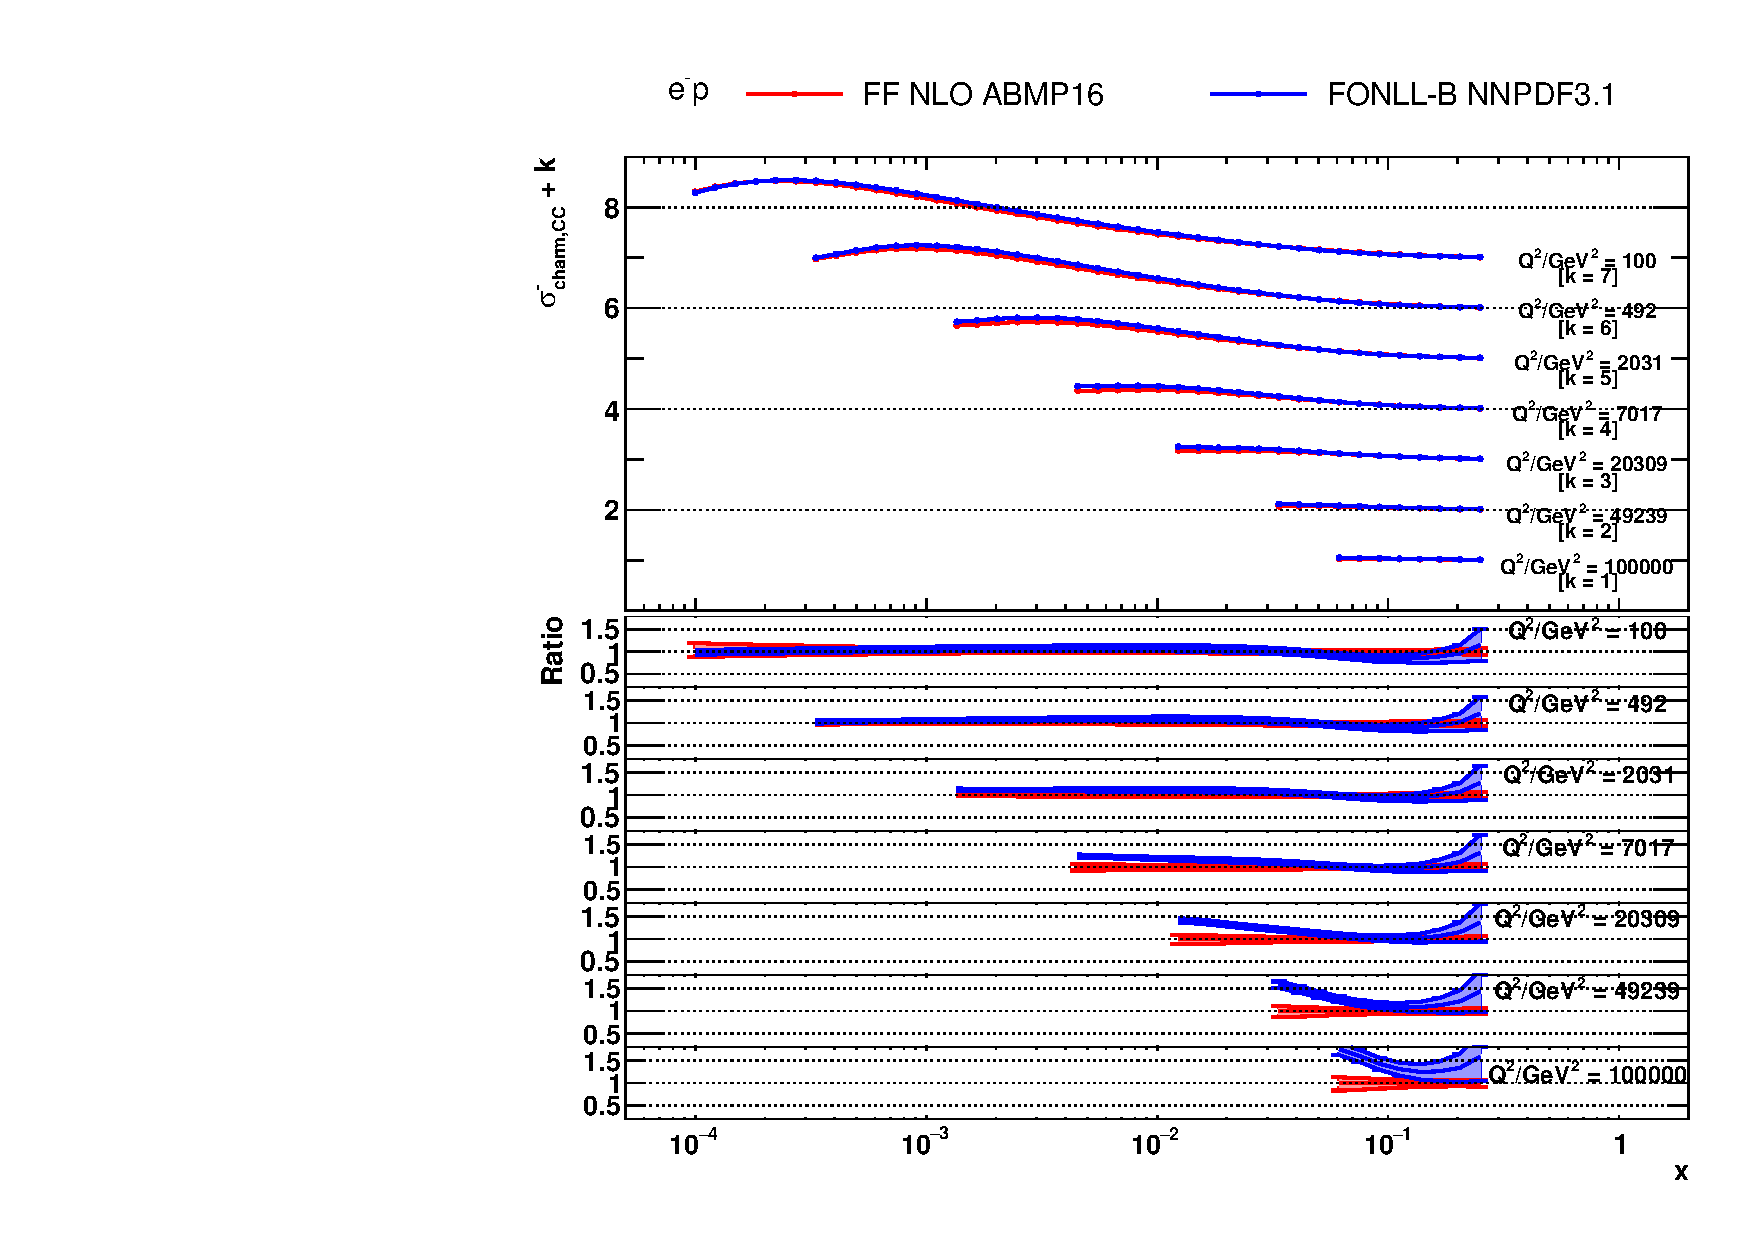
\includegraphics[width=0.50\textwidth]{pics/plots-110818/plot-sigmared-x-em.pdf}}}
    \caption{The theoretical predictions with their total uncertainties for charm CC production at the LHeC as a function of \xbj for different values of $Q^2$ calculated in the \ffns and \fonll schemes. The bottom panel display the theoretical predictions normalised to the nominal values of the \ffns predictions.}
    \label{fig:thpred-x}
\end{figure}

\begin{figure}
    \centering
    \centering{{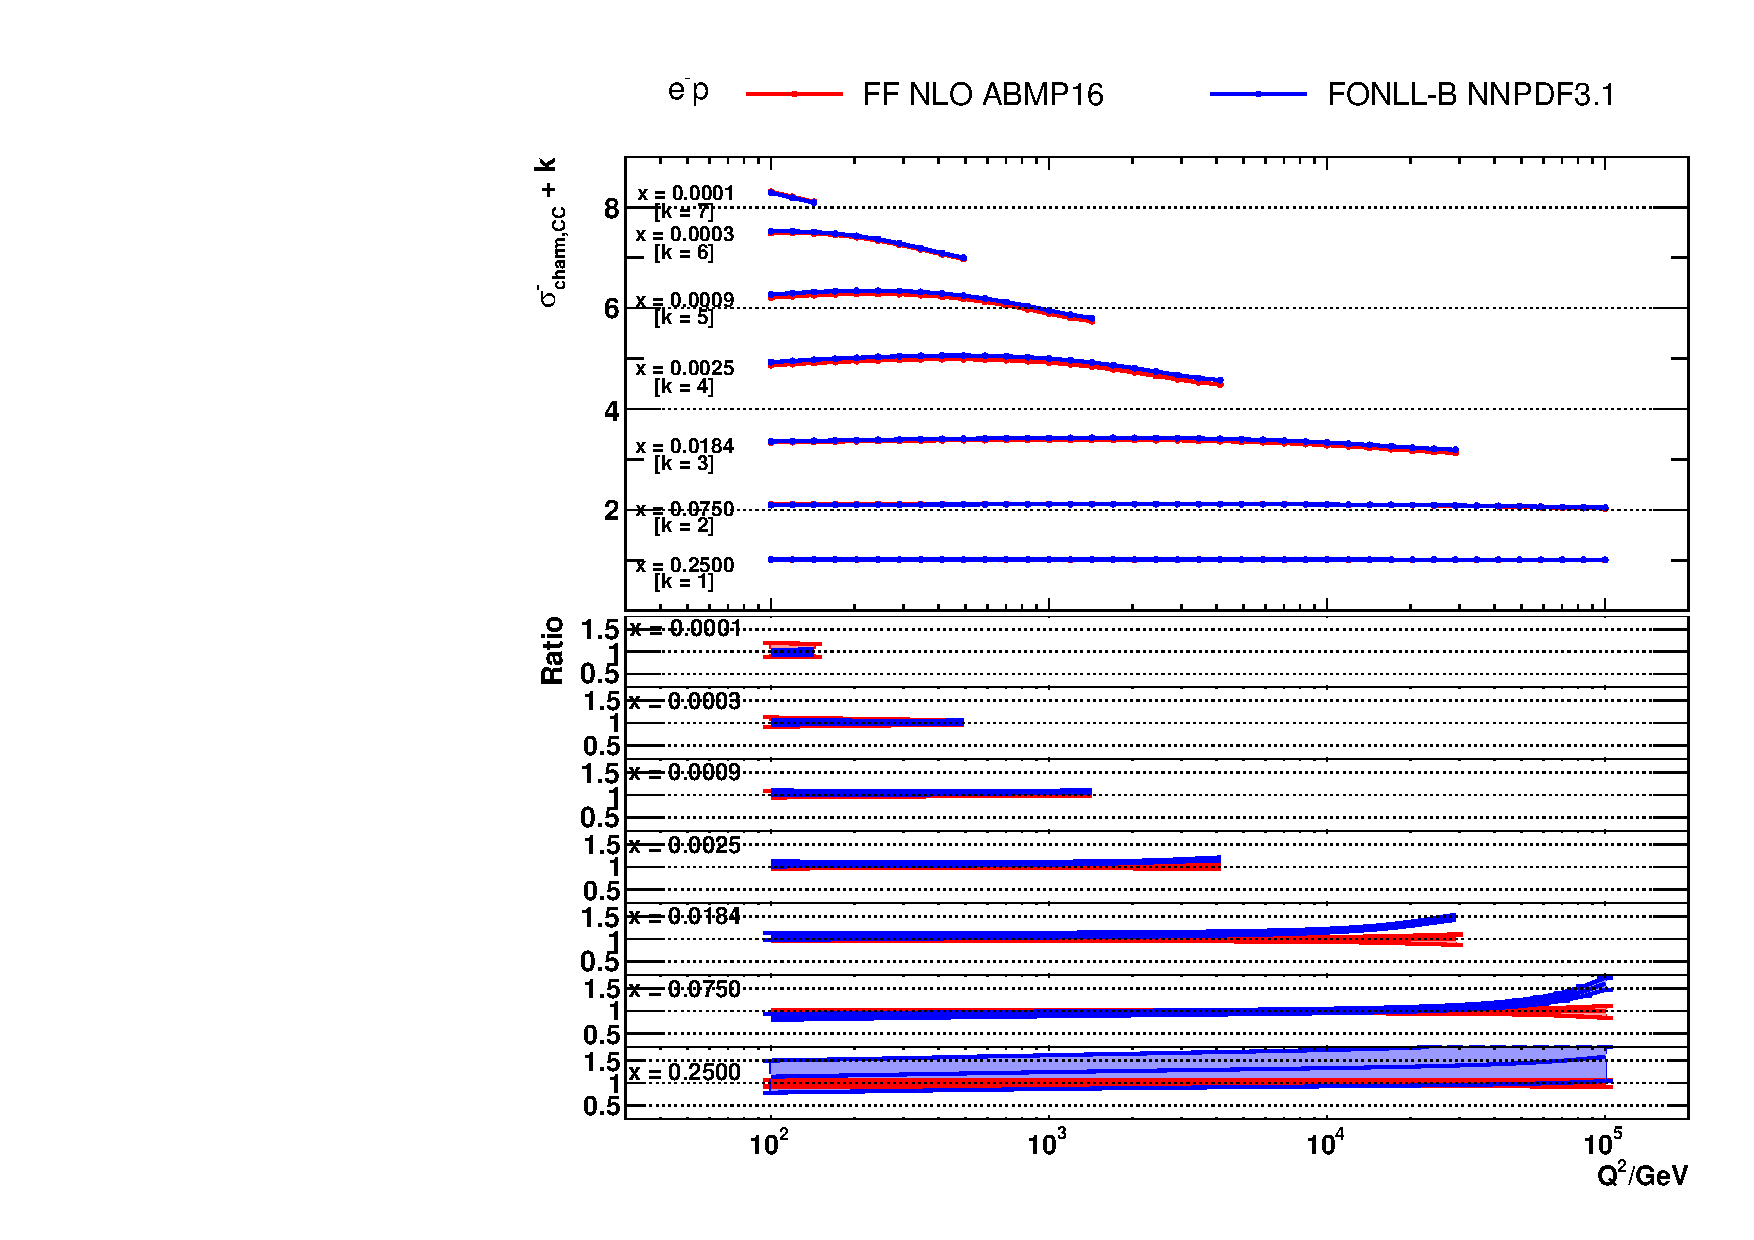
\includegraphics[width=0.50\textwidth]{pics/plots-110818/plot-sigmared-q2-em.pdf}}}
    \caption{The theoretical predictions with their total uncertainties for charm CC production at the LHeC as a function of $Q^2$ for different values of \xbj calculated in the \ffns and \fonll schemes. The bottom panel display the theoretical predictions normalised to the nominal values of the \ffns predictions.}
    \label{fig:thpred-q2}
\end{figure}

\begin{figure}
    \centering
    \centering{{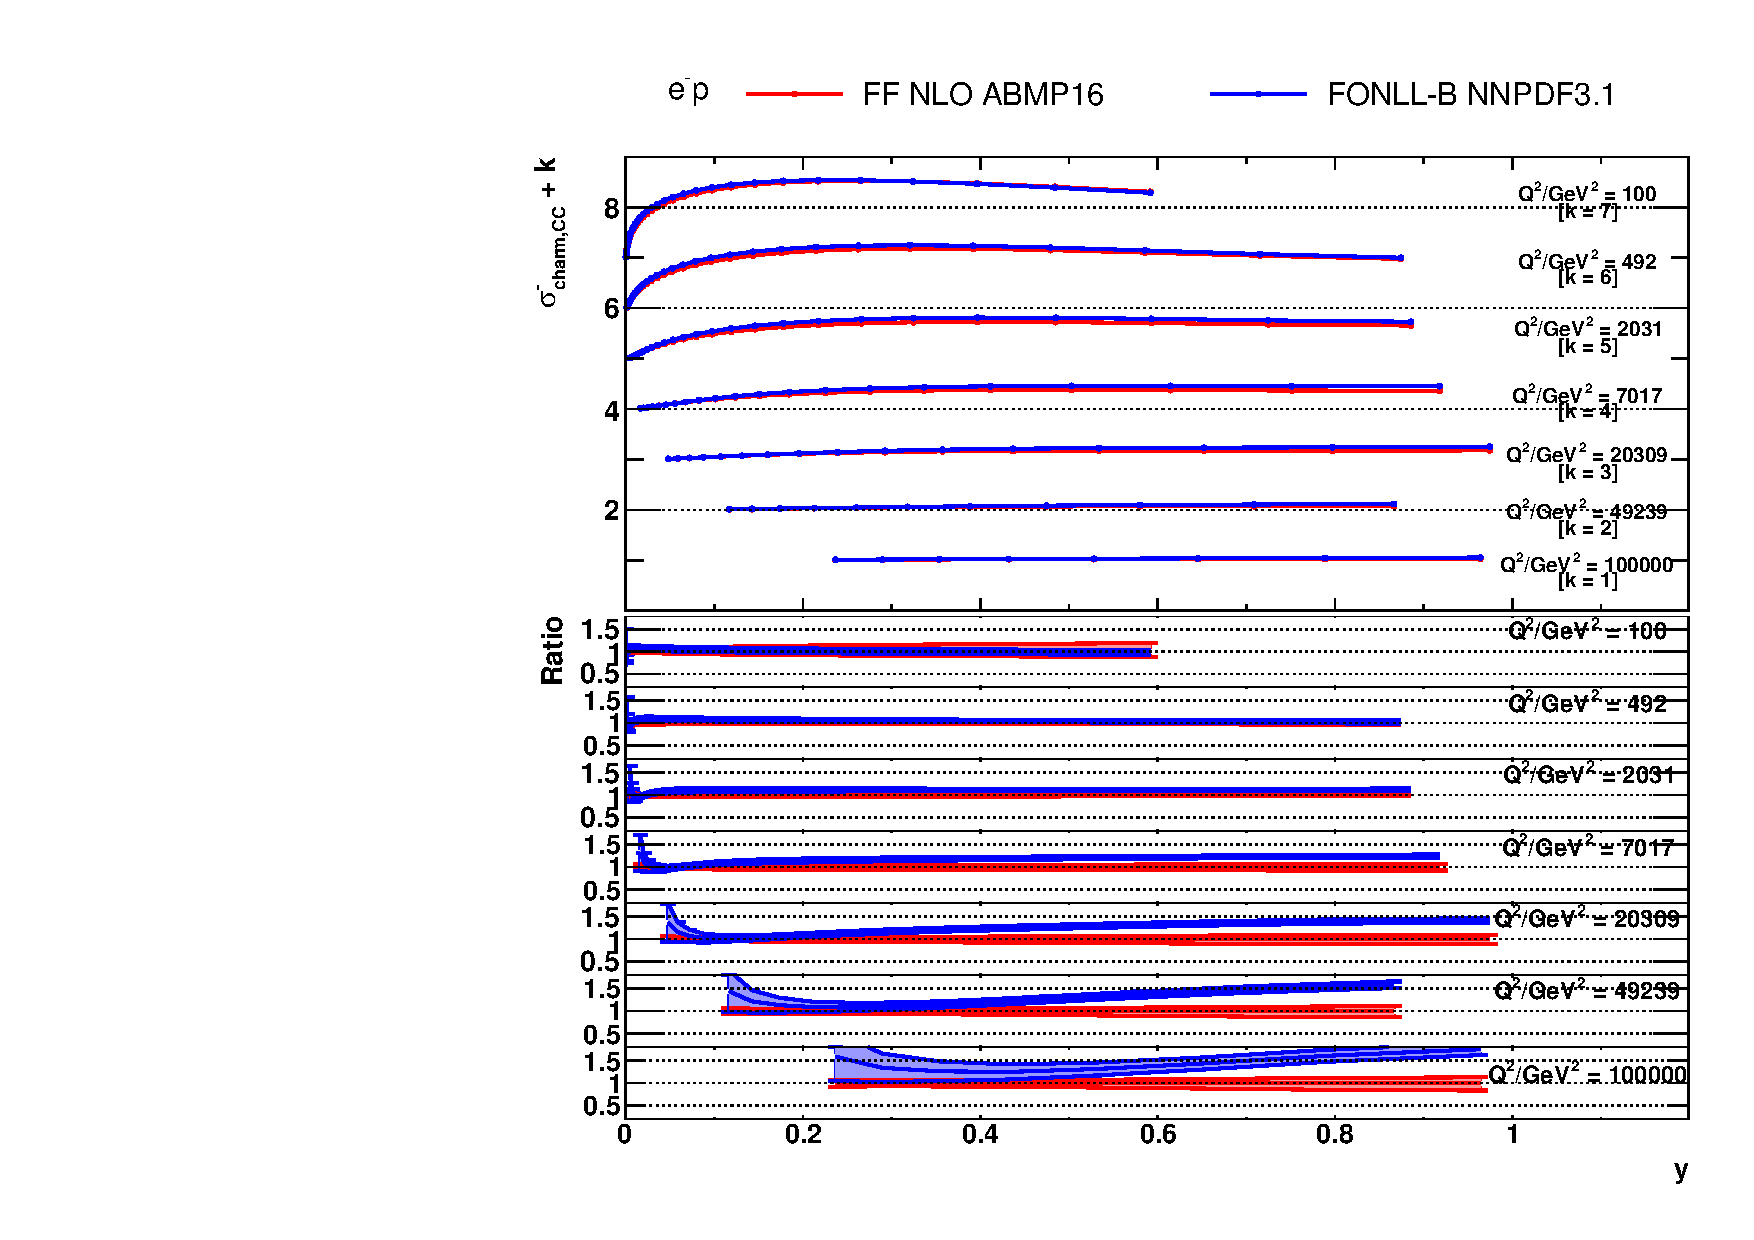
\includegraphics[width=0.50\textwidth]{pics/plots-110818/plot-sigmared-y-em.pdf}}}
    \caption{The theoretical predictions with their total uncertainties for charm CC production at the LHeC as a function of $y$ for different values of $Q^2$ calculated in the \ffns and \fonll schemes. The bottom panel display the theoretical predictions normalised to the nominal values of the \ffns predictions.}
    \label{fig:thpred-y}
\end{figure}

To explore whether the differences between the two sets of theoretical predictions appear due to the different treatment of heavy quarks or due to different PDF sets, theoretical calculations in the \ffns and \fonll schemes are repeated with PDF sets extracted from the fit to the HERA DIS data~\cite{Abramowicz:2015mha}. The fit settings follow the HERAPDF2.0 analysis~\cite{Abramowicz:2015mha}. 
In this study, consistent conditions of the PDF extraction eliminate possible differences between the predictions for the LHeC arising from the dissimilarities of the \abmp and \nnpdf analysis. The obtained results are similar to the ones displayed in Figs.~\ref{fig:thpred-x}--\ref{fig:thpred-y} and prove that these differences arise due to the different treatment of heavy quarks in the two schemes.

Furthermore, to investigate the impact of the NNLO corrections available at $Q \gg m_c$ for the FFNS calculation, approximate NNLO predictions are obtained using the \abmp NNLO PDF set~\cite{Alekhin:2017kpj}. The results for the cross sections as a function of $Q^2$ for difference values of \xbj are shown in Fig.~\ref{fig:thpred-q2-nnlo}, where they are compared to the NLO FFNS predictions from Fig.~\ref{fig:thpred-q2}. The NNLO corrections do not exceed $10\%$ and thus do not cover the differences between the \ffns and \fonll theoretical predictions. Similar results are observed for cross sections as functions of other kinematic variables.

\begin{figure}
    \centering
    \centering{{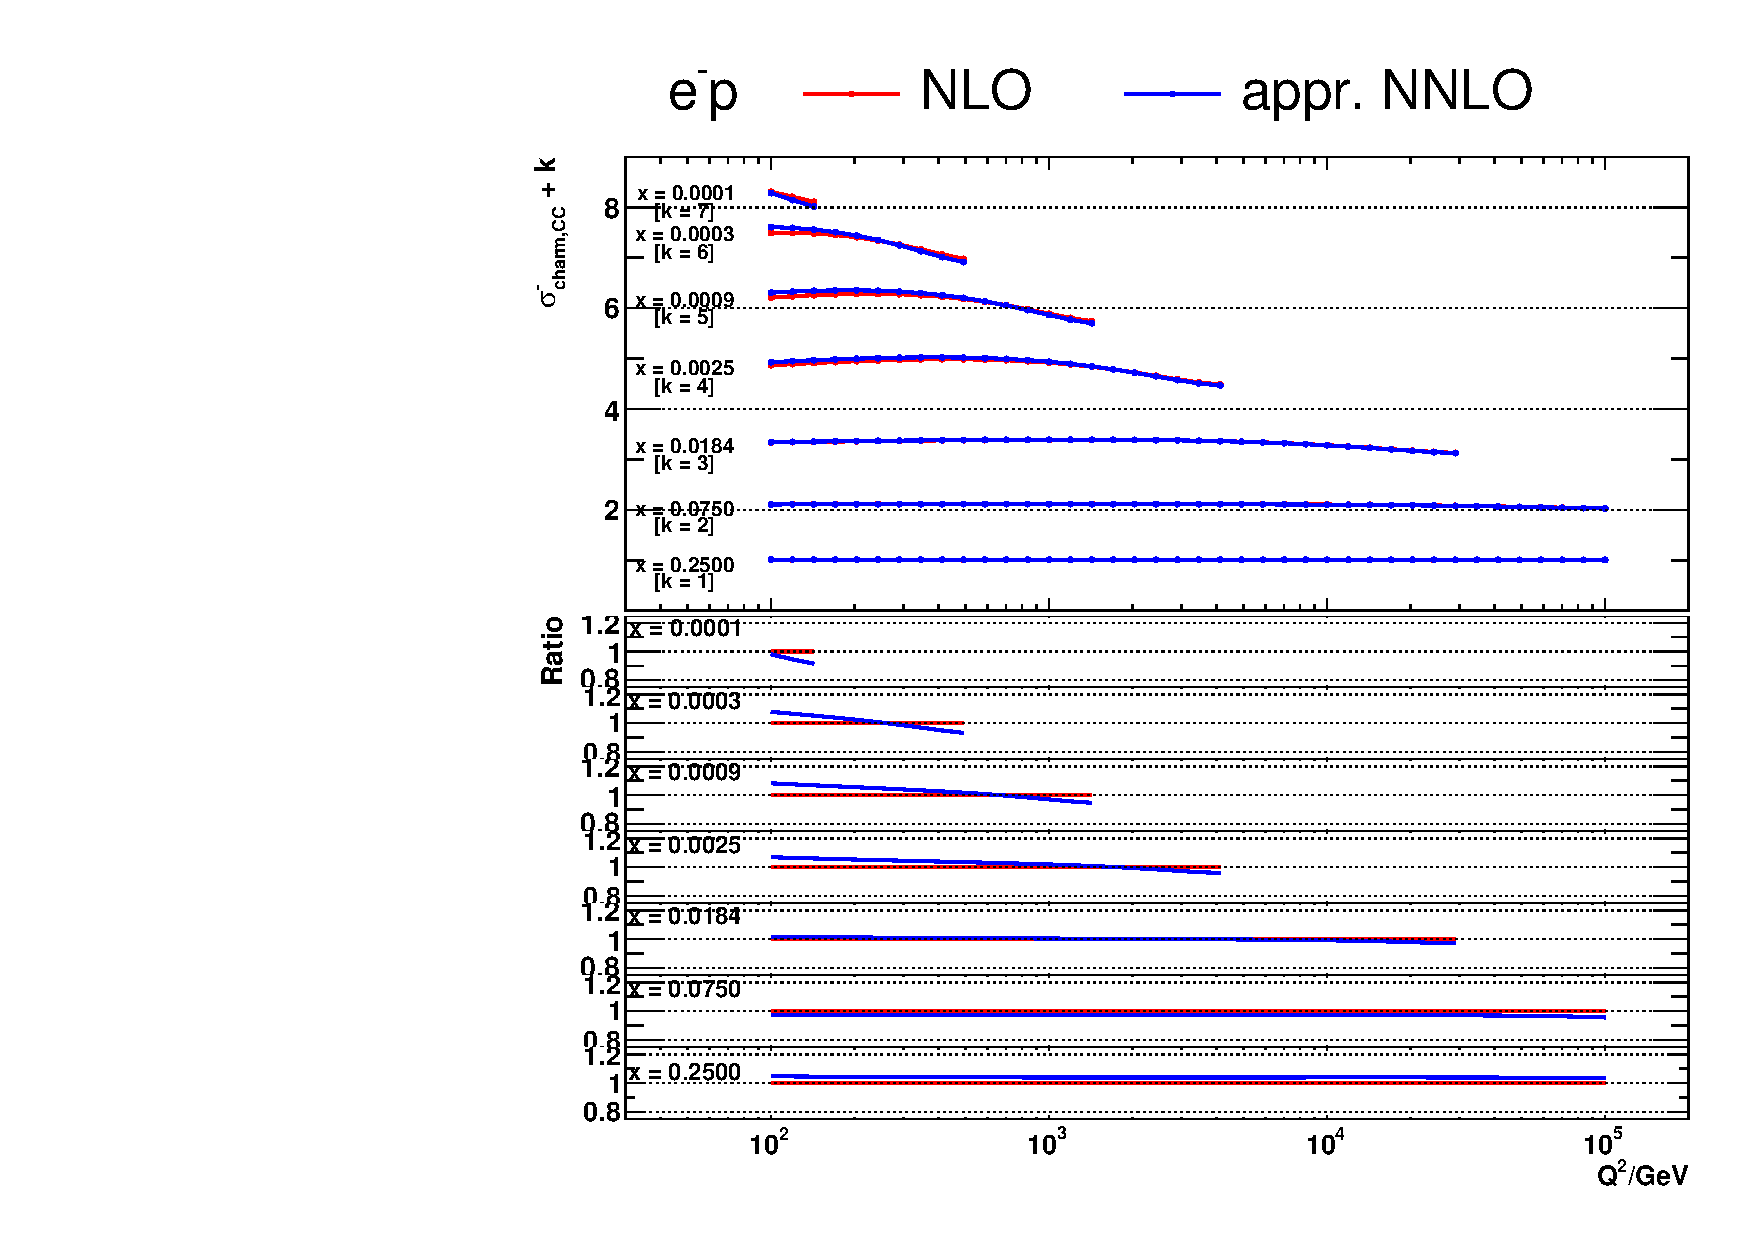
\includegraphics[width=0.50\textwidth]{pics/plots-130918/plot-FFABMnnlo-q2-em.pdf}}}
    \caption{The theoretical predictions with their total uncertainties for charm CC production at the LHeC as a function of $Q^2$ for different values of \xbj calculated in the \ffns scheme at NLO and approximate NNLO. The bottom panel display the theoretical predictions normalised to the nominal values of the \ffns NLO predictions.}
    \label{fig:thpred-q2-nnlo}
\end{figure}

\subsection{Contributions from different partonic subprocesses}
\label{sec:thpred-partonic}

{\bf [perhaps this text would be more appropriate in an earlier theory section]}
The reduced charm CC production cross sections can be expressed as a linear combinations of the structure functions:
\begin{equation}
\begin{split}
    \sigma^{\pm}_{\text{charm,CC}} &= 0.5(Y_{+}F_2^{\pm} \mp Y_{-}xF_3^{\pm} - y^2F_L^{\pm}),\\
    Y_{\pm} &= 1 \pm (1-y)^2.
\end{split}
\end{equation}
In the simplified Quark Parton Model, where gluons are not present, the structure functions become:
\begin{equation}
\begin{split}
    F_2^{+} &= xD + x\overline{U}, \\
    F_2^{-} &= xU + x\overline{D},\\
    F_L &= 0,\\
    xF_3^{+} &= xD - x\overline{U}, \\
    xF_3^{-} &= xU - x\overline{D}.
\end{split}
\end{equation}
The terms $xU$, $xD$, $x\overline{U}$ and $x\overline{D}$ denote the sums of parton distributions for up-type and down-type quarks and anti-quarks, respectively. 
Below the $b$-quark mass threshold, these sums are related to the quark distributions as follows:
\begin{equation}
\begin{split}
 xU &= xu + xc , \\
 x\overline{U} &= x\overline{u} + x\overline{c} , \\
 xD &= xd + xs , \\
 x\overline{D} &= x\overline{d} + x\overline{s}.
\end{split}
\end{equation}
In the FFNS the charm quark density is zero.
In the phase space corners $y \to 0$ and $y \to 1$, the following assymptotics take place:
\begin{equation}
\begin{split}
 y \to 0: \sigma^{\pm}_{\text{charm,CC}} &= F_2^{\pm} = xD(x\overline{D}) + xU(x\overline{U}), \\
 y \to 1: \sigma^{\pm}_{\text{charm,CC}} &= 0.5(F_2^{\pm} \mp xF_3^{\pm}) = xU (x\overline{U}).
\label{eq:y01}
\end{split}
\end{equation}
Thus the contribution from the strange quark PDF is suppressed at high $y$.

Figures~\ref{fig:partonic-x}, \ref{fig:partonic-q2} and \ref{fig:partonic-y} show contributions from different partonic subprocesses for charm CC production cross sections in the \ffns and \fonll schemes as a function of \xbj for different values of $Q^2$, as a function of $Q^2$ for different values of \xbj, and as a function of $y$ for different values of $Q^2$, respectively.
In both scheme, the strange quark PDF contibutes only about $50\%$ to total charm CC production. In particular, at high $y$ its contribution drops to zero in favour of the gluon or charm quark PDF (see Fig.~\ref{fig:partonic-y} and Eq.~\ref{eq:y01}). Similar phenomena (although less pronounced) is observed at low \xbj and/or high $Q^2$. In these phase space regions, the dominant contributions to the cross sections are the gluon PDF (in the FFNS) or the charm quark PDF (in the VFNS). Remarkably, these contributions as functions of $Q^2$, \xbj and $y$ behave qualitatively very similar in the FFNS and VFNS.

\begin{figure*}
    \centering
    \centering{{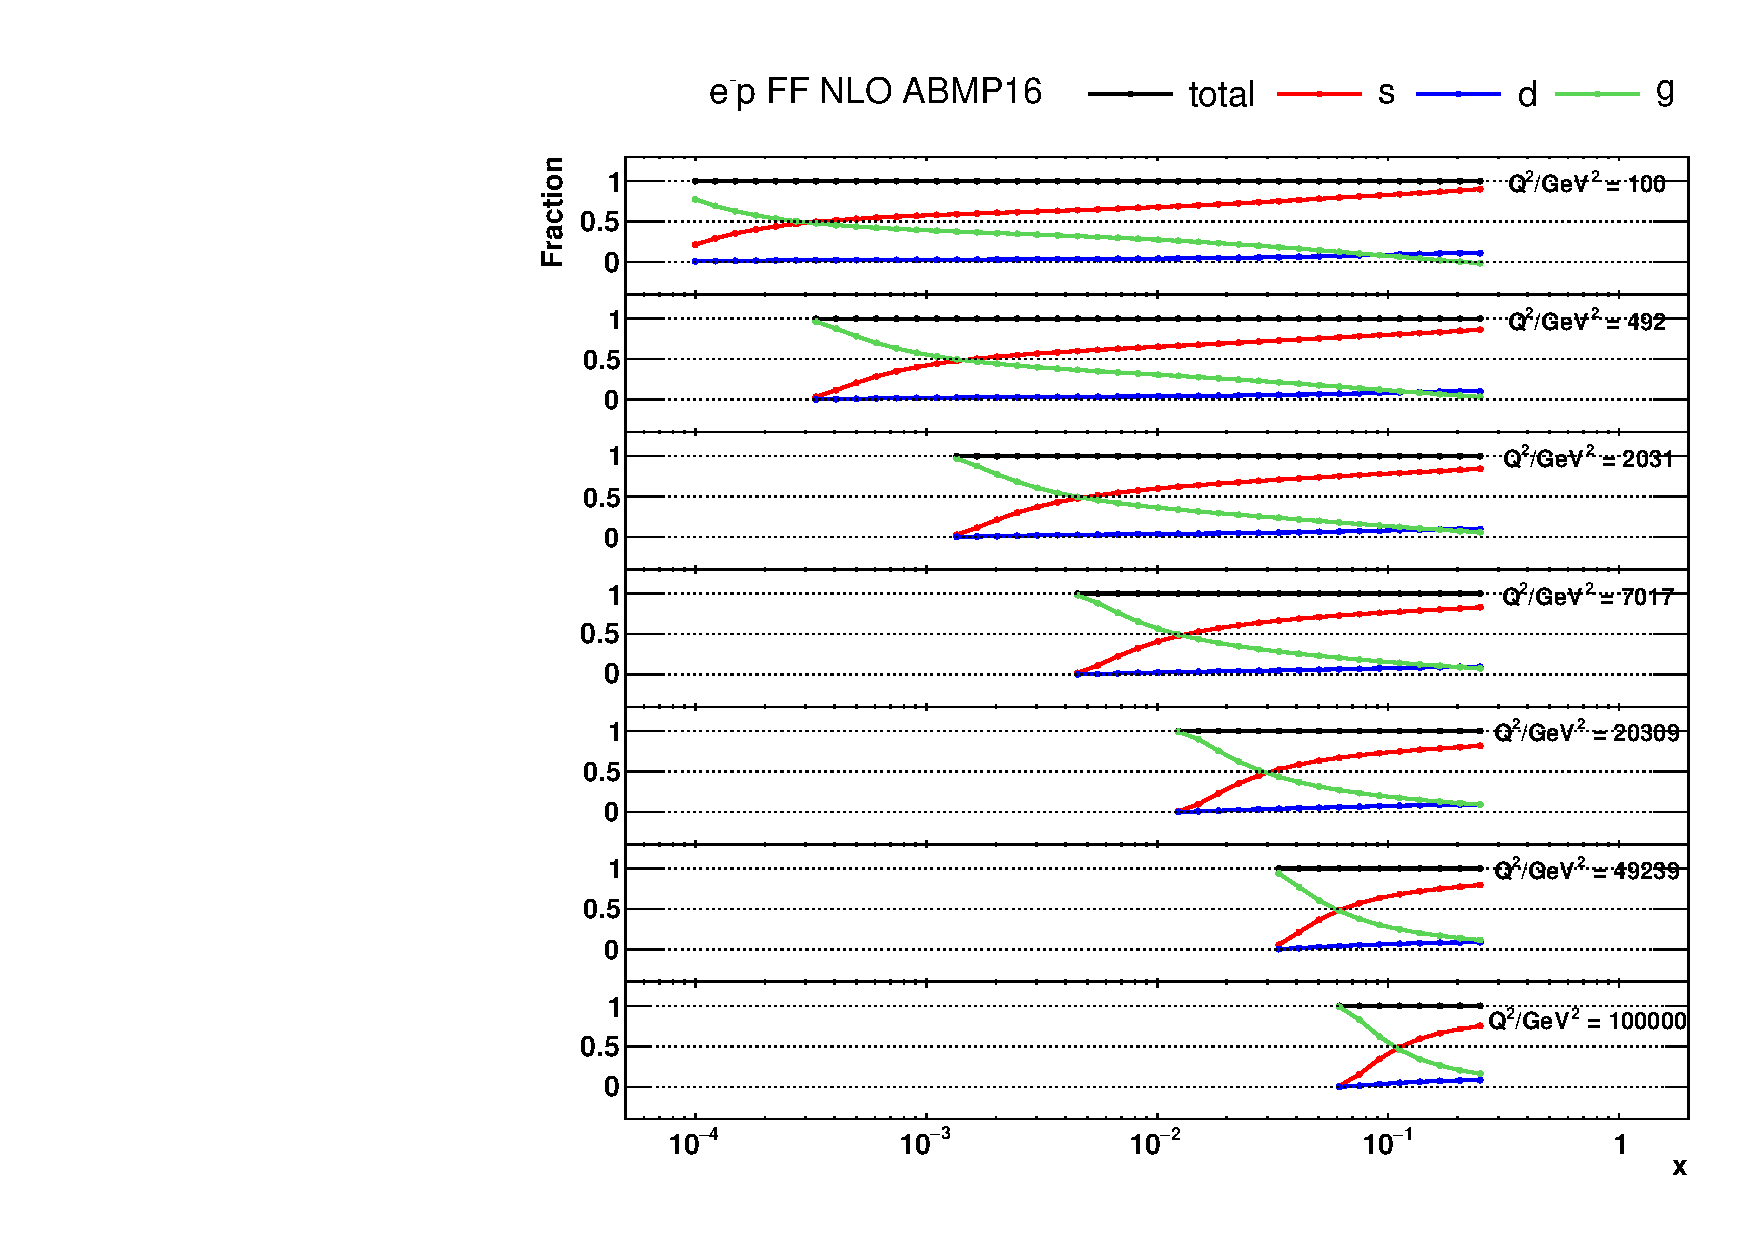
\includegraphics[width=0.49\textwidth]{pics/plots-110818/plot-parton-x-em-FFABM.pdf}}}
    \centering{{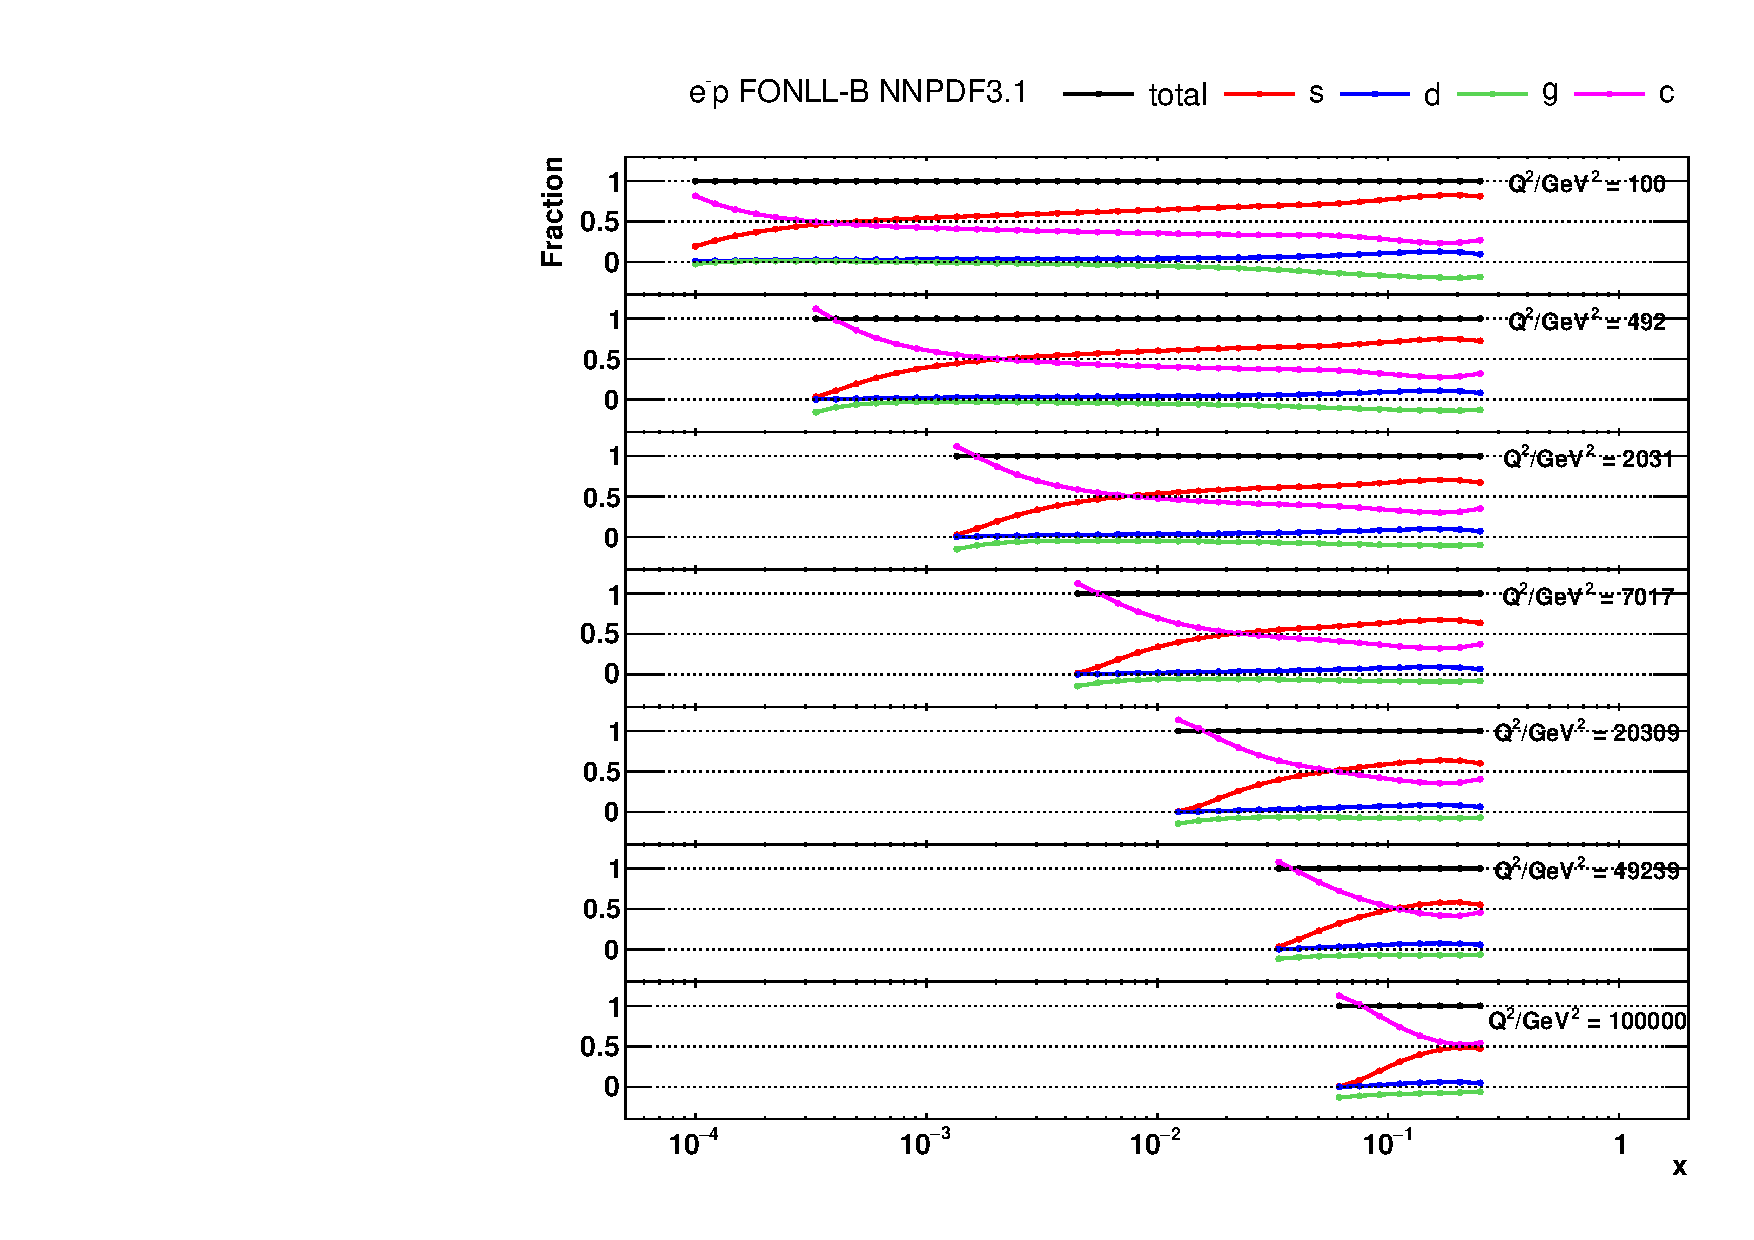
\includegraphics[width=0.49\textwidth]{pics/plots-110818/plot-parton-x-em-FONLL.pdf}}}
    \caption{The partonic subprocesses for charm CC production cross sections in the \ffns (left) and \fonll (right) schemes as a function of \xbj for different values of $Q^2$.}
    \label{fig:partonic-x}
\end{figure*}

\begin{figure*}
    \centering
    \centering{{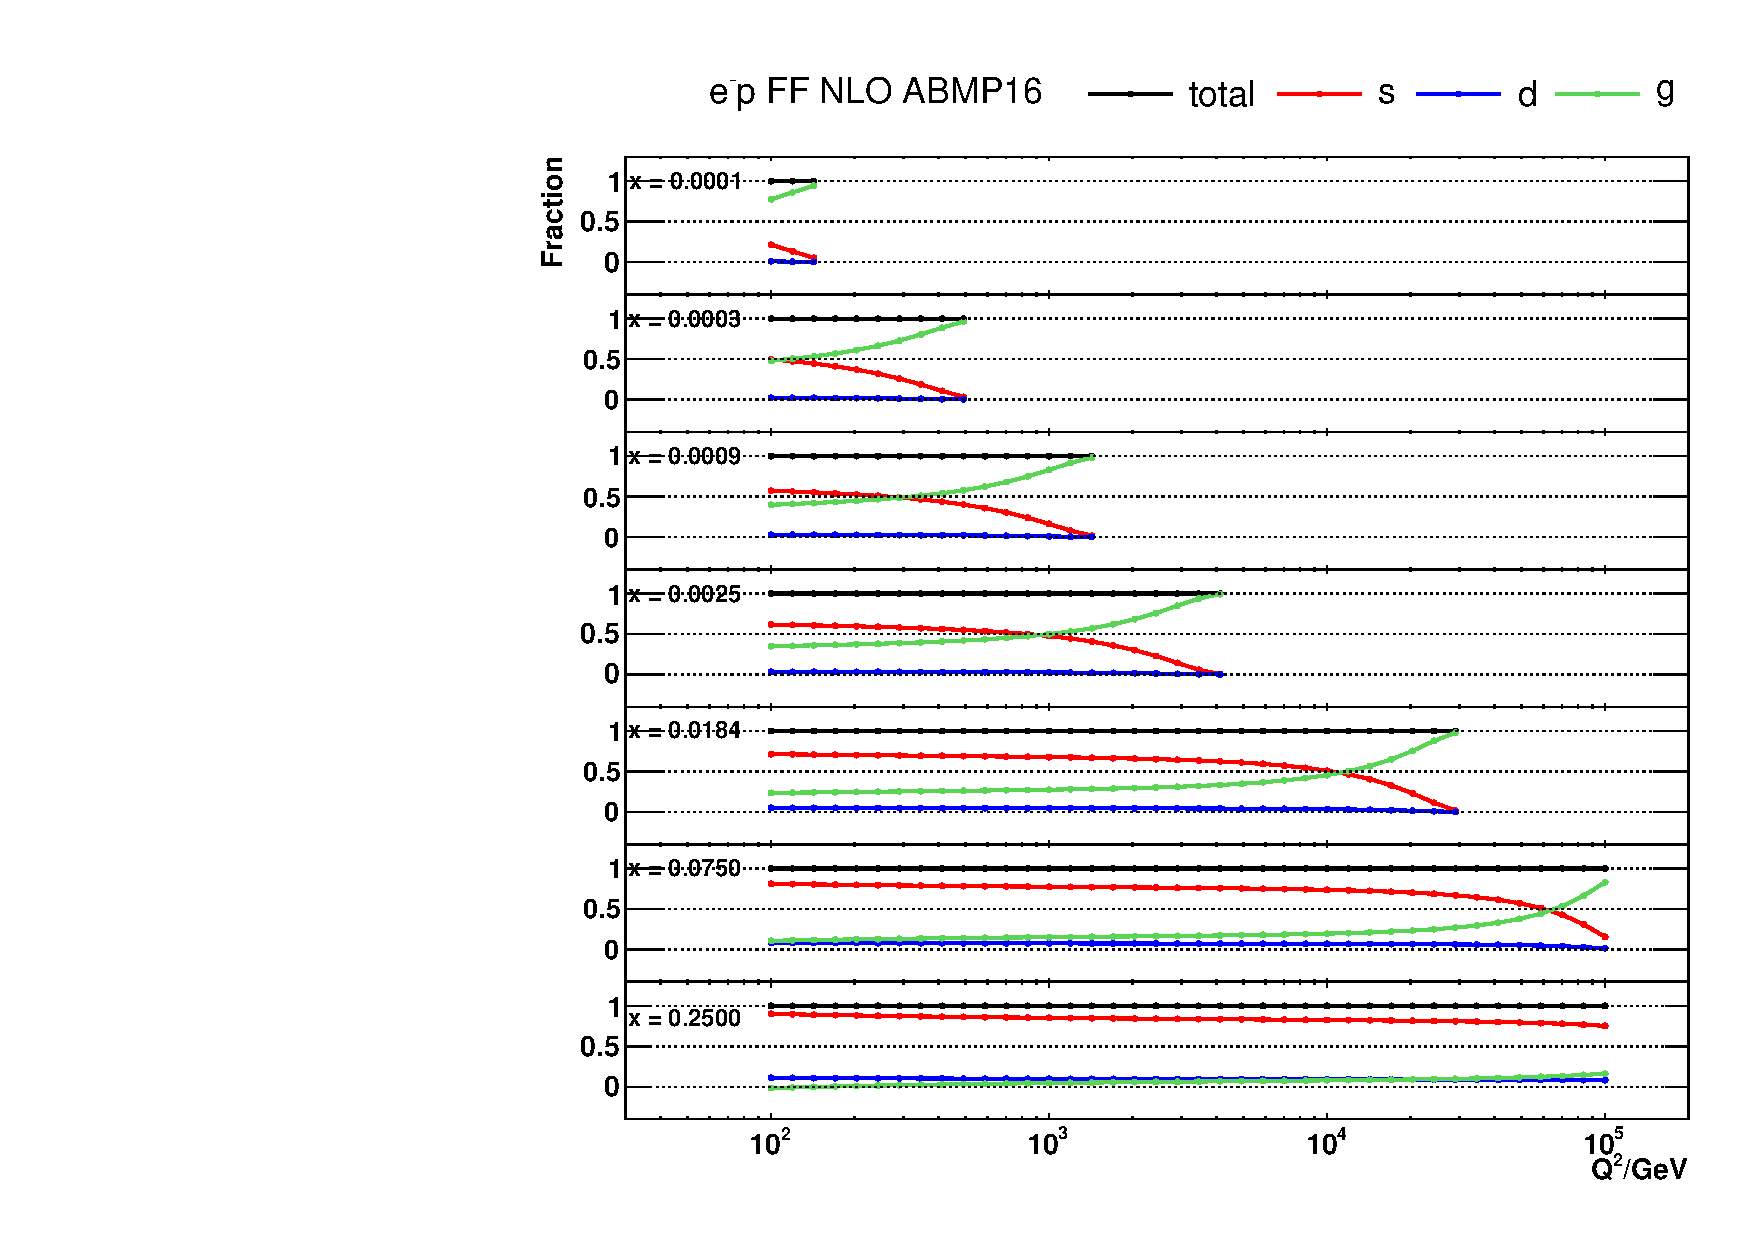
\includegraphics[width=0.49\textwidth]{pics/plots-110818/plot-parton-q2-em-FFABM.pdf}}}
    \centering{{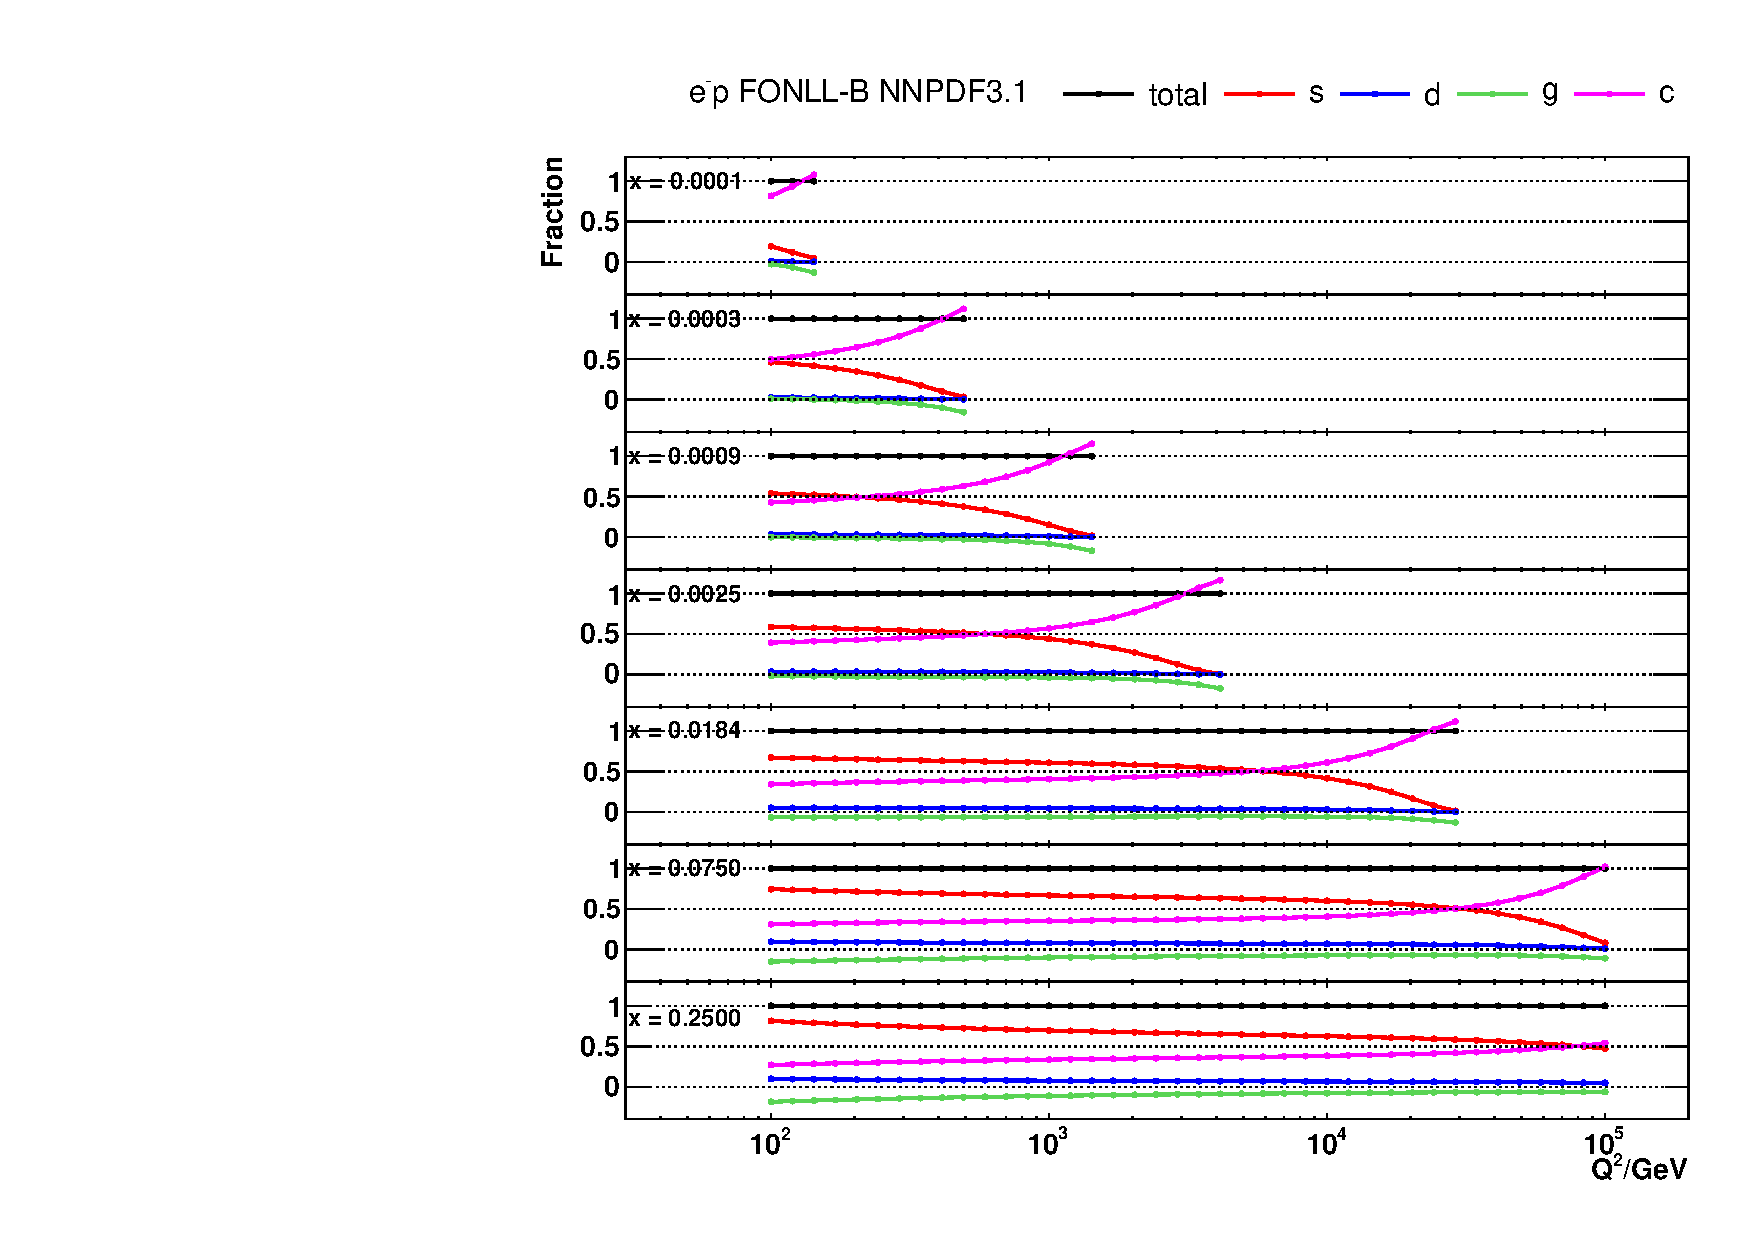
\includegraphics[width=0.49\textwidth]{pics/plots-110818/plot-parton-q2-em-FONLL.pdf}}}
    \caption{The partonic subprocesses for charm CC production cross sections in the \ffns (left) and \fonll (right) schemes as a function of $Q^2$ for different values of \xbj.}
    \label{fig:partonic-q2}
\end{figure*}

\begin{figure*}
    \centering
    \centering{{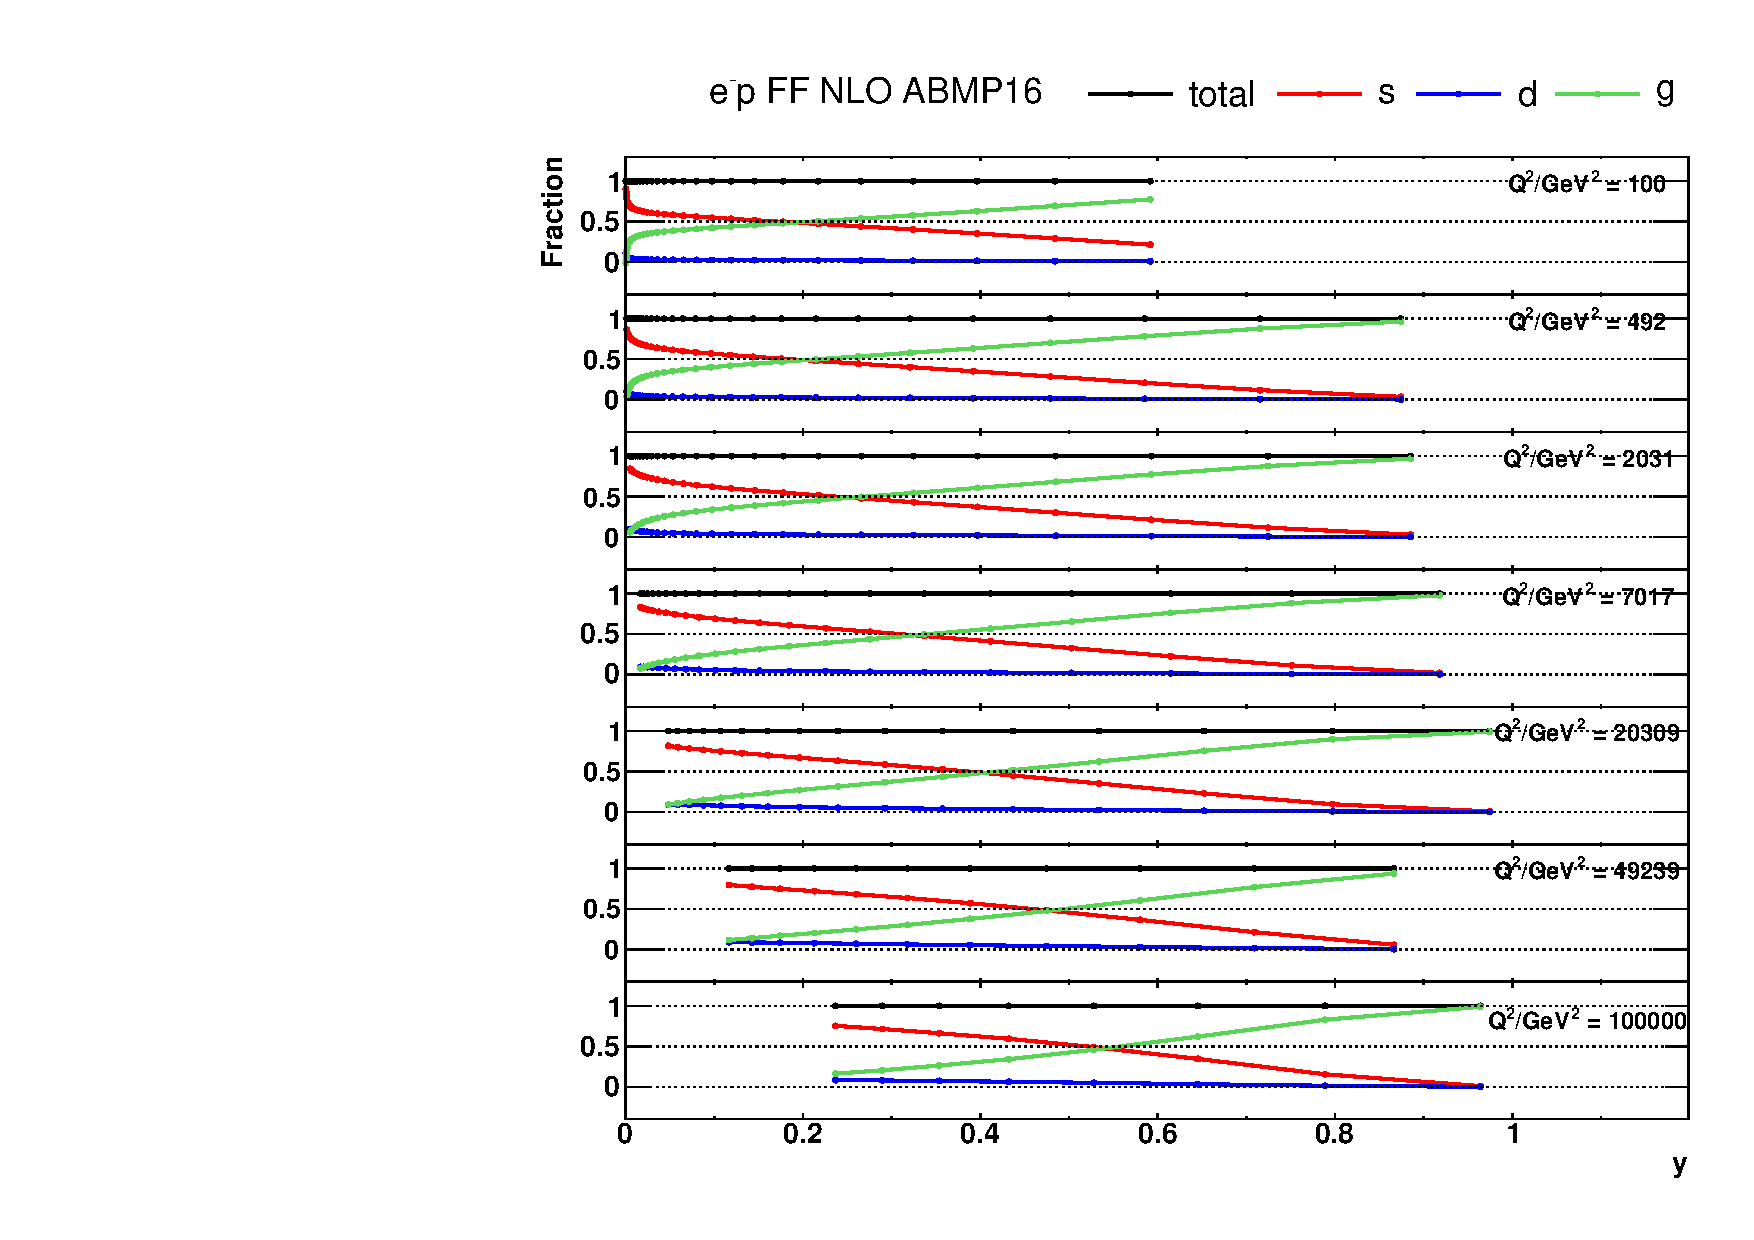
\includegraphics[width=0.49\textwidth]{pics/plots-110818/plot-parton-y-em-FFABM.pdf}}}
    \centering{{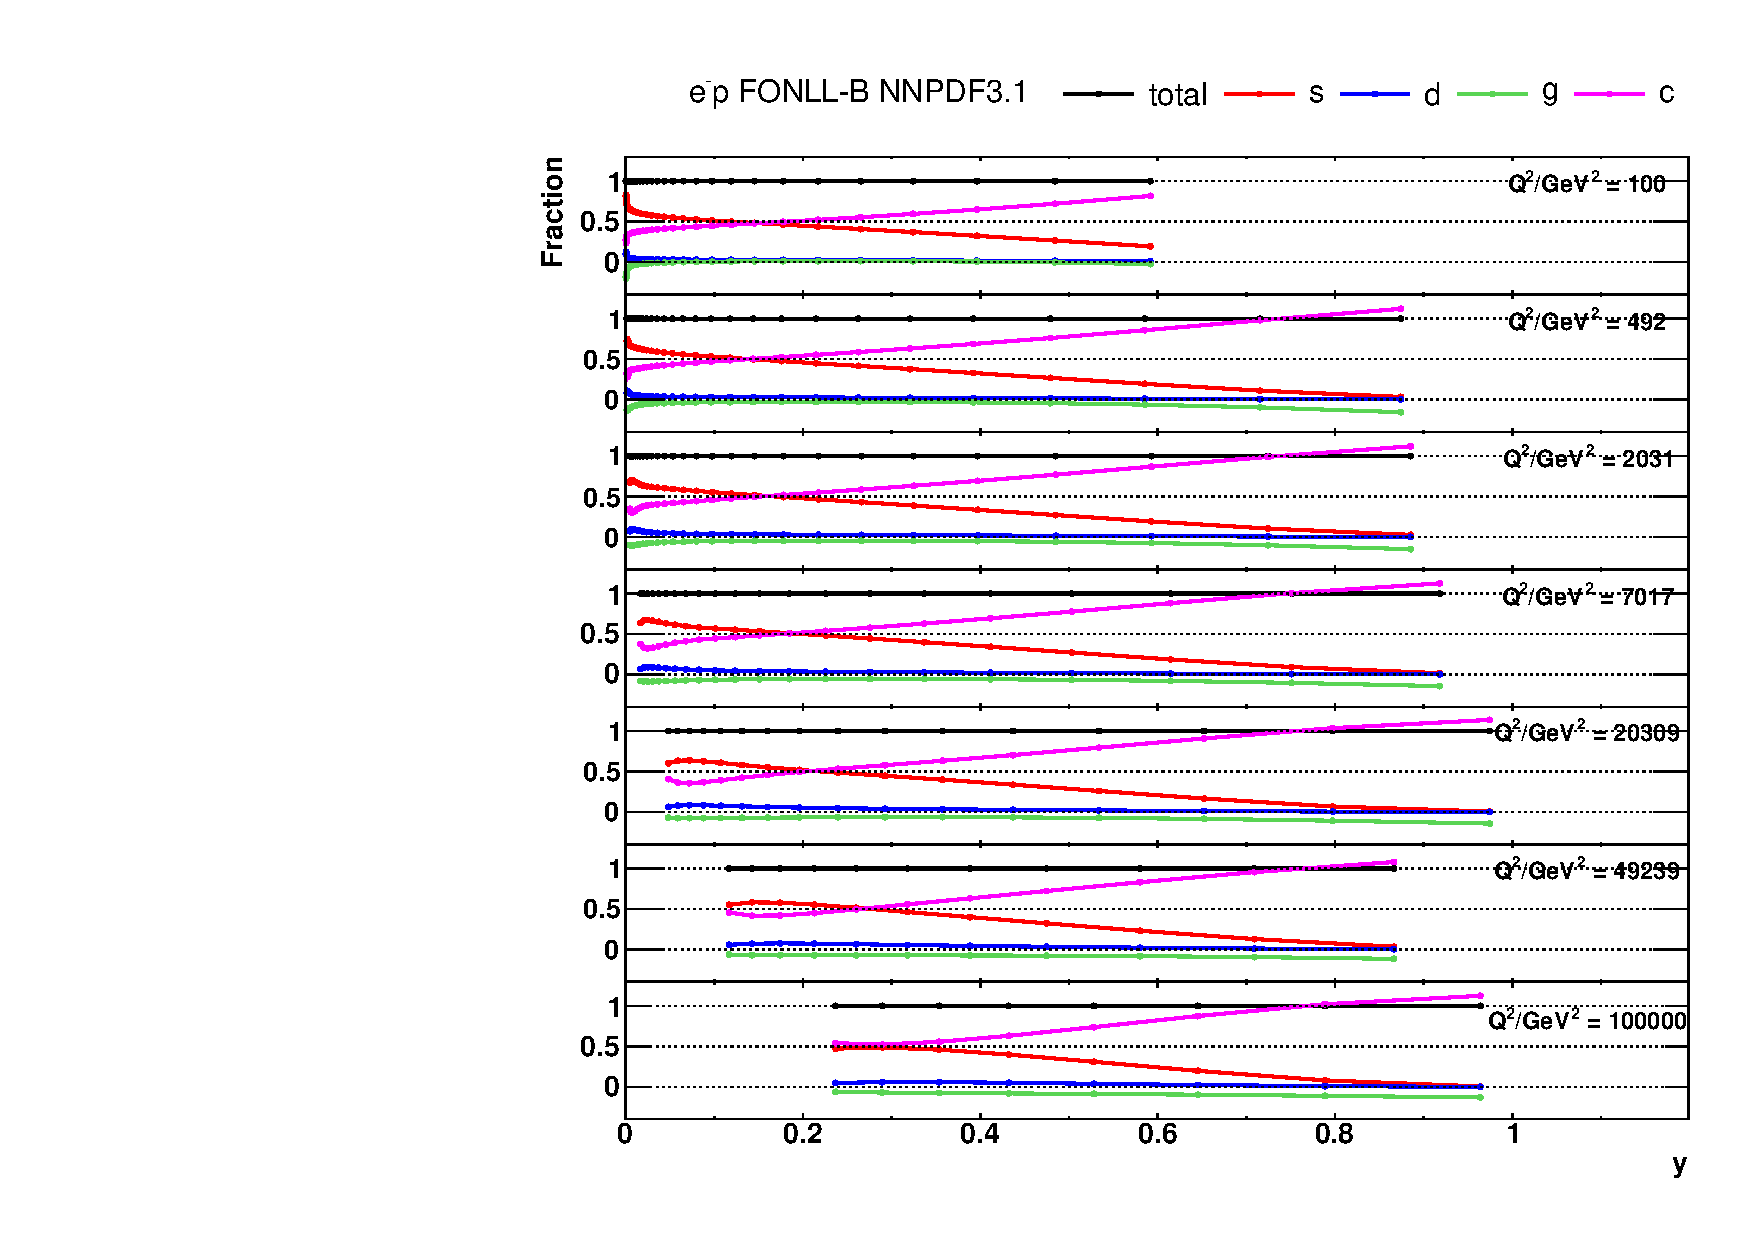
\includegraphics[width=0.49\textwidth]{pics/plots-110818/plot-parton-y-em-FONLL.pdf}}}
    \caption{The partonic subprocesses for charm CC production cross sections in the \ffns (left) and \fonll (right) schemes as a function of $y$ for different values of $Q^2$.}
    \label{fig:partonic-y}
\end{figure*}

\section{PDF constraints from charm CC pseudodata}
\label{sec:PDF}

The impact of charm CC cross section measurements at the LHeC on the PDFs is quantitatively estimated using a profiling technique~\cite{Paukkunen:2014zia}. This technique is based on minimising \chisq between data and theoretical predictions taken into account both experimental and theoretical uncertainties arising from PDF variations. Two NLO PDF sets were chosen for this study: 
\abmp~\cite{Alekhin:2018pai} and \nnpdf~\cite{Ball:2017nwa} available via the \lhapdf interface (version 6.1.5)~\cite{Buckley:2014ana}. 
All PDF sets are provided with uncertainties in the format of eigenvectors. 

For this study, pseudodata representing measurements of charm CC production cross sections as a function of $Q^2$ and $x$ are used. {\bf [TODO: describe how pseudodata were produced]}
The study is performed using the \xfitter program (version 2.0.0)~\cite{Alekhin:2014irh}, an open-source QCD fit framework for PDF determination. The theoretical predictions are calculated at NLO QCD in the FFNS with the number of active flavours $n_f = 3$ and FONLL-B with $n_f = 5$. The running charm mass is set to $m_c(m_c) = 1.27$ GeV and $\alpha_s$ is set to the value used for the corresponding PDF extraction.
The renormalisation and factorisation scales are chosen to be $\mu_\mathrm{r} = \mu_\mathrm{f} = Q^2$.

The \chisq value is calculated as follows:
\begin{equation}
\chisq = \mathbf{R}^{T}_{} \mathbf{Cov}^{-1}_{} \mathbf{R}_{} + \sum_{\beta} b_{\beta,\rm th}^2,~~~\mathbf{R} = \mathbf{D} - \mathbf{T} - \sum_{\beta} \Gamma^{}_{\beta,\rm th} b_{\beta,\rm th},
\label{eq:chisq}
\end{equation}

where $\mathbf{D}$ and $\mathbf{T}$ are the column vectors of the measured and predicted values, respectively, 
and the correlated theoretical PDF uncertainties are included using the nuisance parameter vector $\boldsymbol{b_{\rm th}}$ with their influence on the theory predictions described by $\Gamma^{}_{\beta,\rm th}$, where index $\beta$ runs over all PDF eigenvectors. 
For each nuisance parameter a penalty term is added to the \chisq, representing the prior knowledge of the parameter. 
No theoretical uncertainties except the PDF uncertainties are considered.
The full covariance matrix representing the statistical and systematic uncertainties of the data is used in the fit. The statistical and systematic uncertainties are treated as additive, i.e., they do not change in the fit. The systematic uncertainties are assumed uncorrelated between bins.

To treat the asymmetric PDF uncertainties of the \nnpdf set, the \chisq function in Eq.~\ref{eq:chisq} is generalised assuming a parabolic dependence of the prediction on the nuisance parameter~\cite{Alekhin:2014irh}:
\begin{eqnarray}
\Gamma^{}_{\beta, \rm th} \to \Gamma^{}_{\beta, \rm th} +  \Omega^{}_{\beta, \rm th}b_{\beta, \rm th}\,, \label{eq:iter}
\end{eqnarray}
where $\Gamma^{}_{\beta, \rm th} = 0.5(\Gamma^{+}_{\beta, \rm th} - \Gamma^{-}_{\beta, \rm th})$ and $\Omega^{}_{\beta} = 0.5(\Gamma^{+}_{\beta, \rm th}
+ \Gamma^{-}_{\beta, \rm th})$ are determined from the shifts of predictions corresponding to up ($\Gamma^{+}_{\beta, \rm th}$) and down ($ \Gamma^{-}_{\beta, \rm th}$) PDF uncertainty eigenvectors.

The values of the nuisance parameters at the minimum, $b^{\rm min}_{\beta,\rm th}$ are interpreted as optimised, or profiled, PDFs, while their uncertainties determined using the tolerance criterion of $\Delta\chi^2 = 1$ correspond to the new PDF uncertainties. The profiling approach assumes that the new data are compatible with theoretical predictions using the existing PDFs, such that no modification of the PDF fitting procedure is needed. Under this assumption, the central values of the measured cross sections are set to the central values of the theoretical predictions. 

The original and profiled \abmp and \nnpdf PDF uncertainties are shown in Figs.~\ref{fig:pdf-abmp}--\ref{fig:pdf-nnpdf-100000}. 
The uncertainties of the PDFs are presented at the scales $\mu_\mathrm{f}^2=100$ GeV$^2$ and $\mu_\mathrm{f}^2=100000$ GeV$^2$.
A strong impact of the charm CC pseudodata on the PDFs is observed for both PDF sets.
In particular, the uncertainties of the strange PDF are strongly reduced once the pseudodata are included in the fit. 
Also the gluon PDF uncertainties are decreased. Furthermore, in the case of the NNPDF3.1 set and FONLL scheme, the charm PDF uncertinties are reduced significantly.

\begin{figure}
    \centering
    {{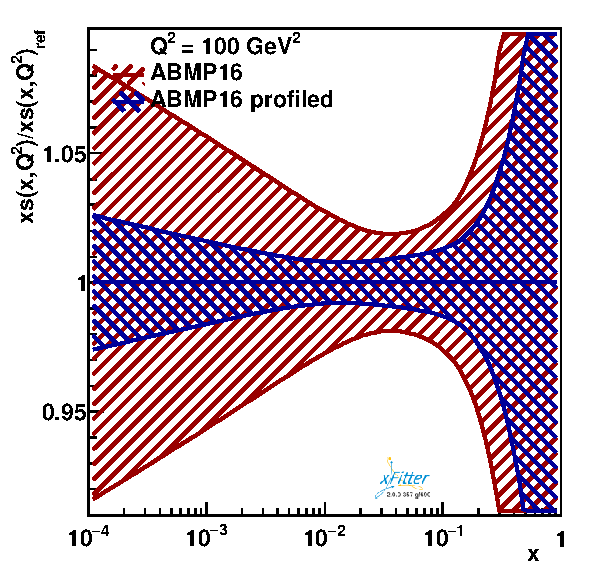
\includegraphics[width=0.235\textwidth]{pics/pdf-profile-ffabm/q2_100_pdf_s_ratio.pdf}}}
    {{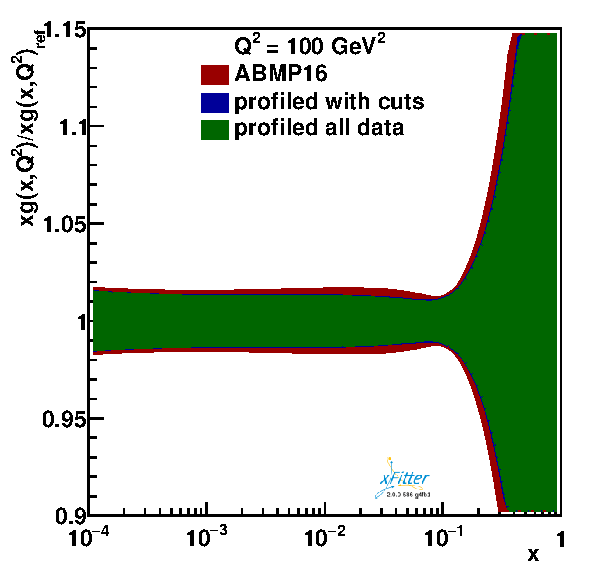
\includegraphics[width=0.235\textwidth]{pics/pdf-profile-ffabm/q2_100_pdf_g_ratio.pdf}}}\\
    {{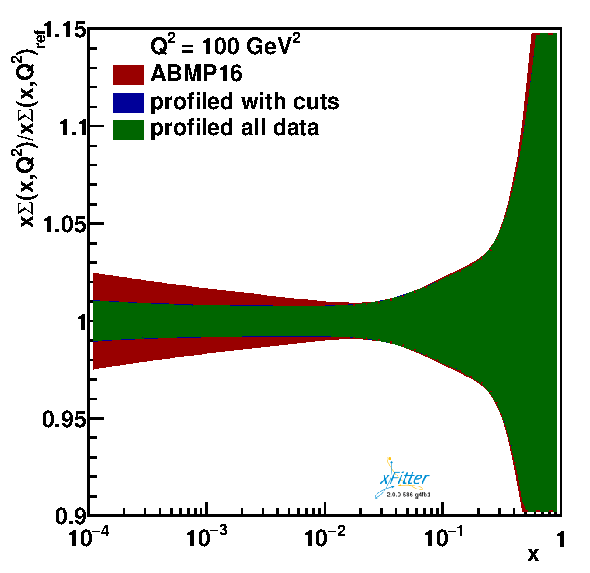
\includegraphics[width=0.235\textwidth]{pics/pdf-profile-ffabm/q2_100_pdf_Sea_ratio.pdf}}}
    {{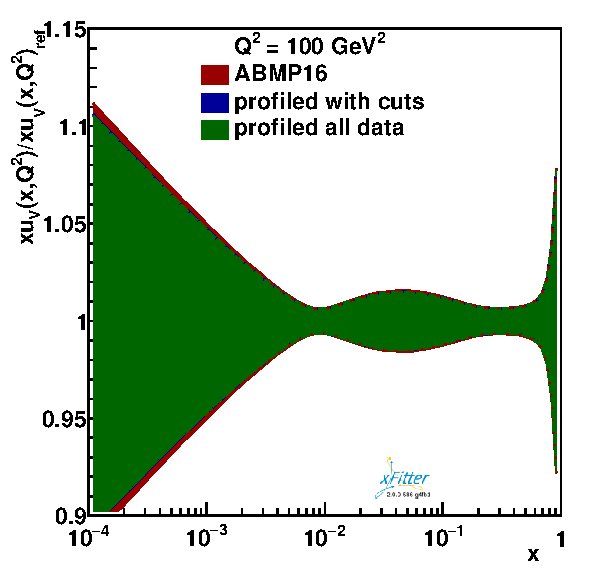
\includegraphics[width=0.235\textwidth]{pics/pdf-profile-ffabm/q2_100_pdf_uv_ratio.pdf}}}
    {{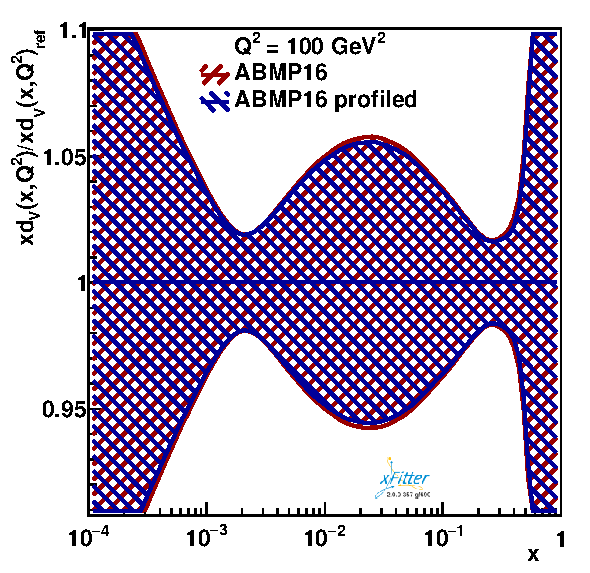
\includegraphics[width=0.235\textwidth]{pics/pdf-profile-ffabm/q2_100_pdf_dv_ratio.pdf}}}
    \caption{The relative strange (top left), gluon (top right), sea quark (middle left), u valence quark (middle right) and d valence quark (bottom) PDF uncertainties at $\mu_\mathrm{f}^2=100$ GeV$^2$ of the original and profiled \abmp PDF set.}
    \label{fig:pdf-abmp}
\end{figure}

\begin{figure}
    \centering
    {{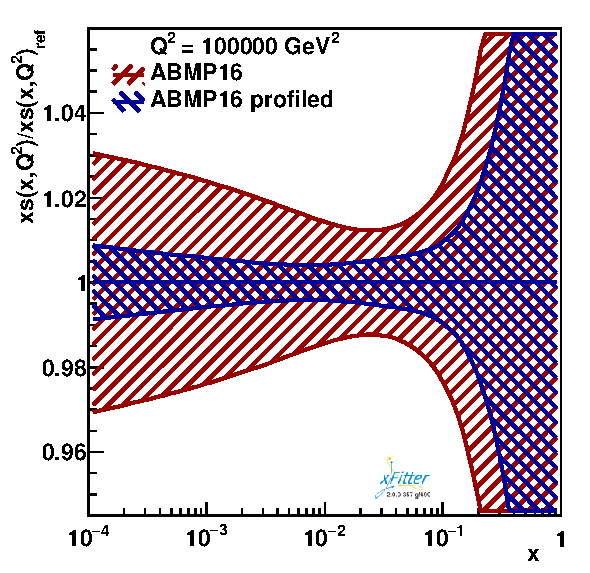
\includegraphics[width=0.235\textwidth]{pics/pdf-profile-ffabm/q2_100000_pdf_s_ratio.pdf}}}
    {{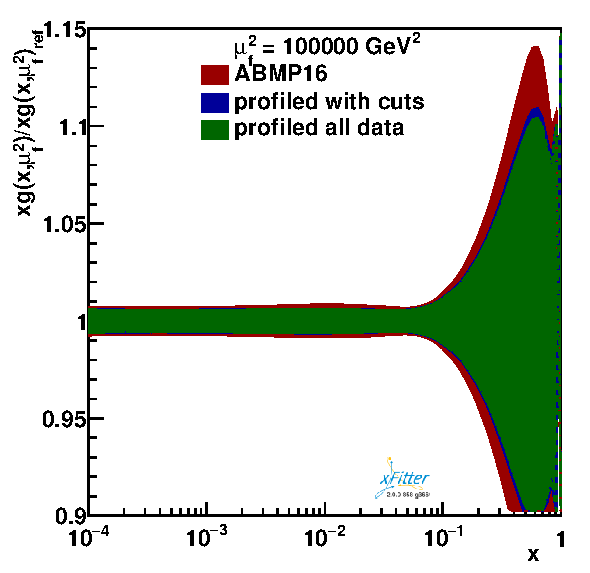
\includegraphics[width=0.235\textwidth]{pics/pdf-profile-ffabm/q2_100000_pdf_g_ratio.pdf}}}\\
    {{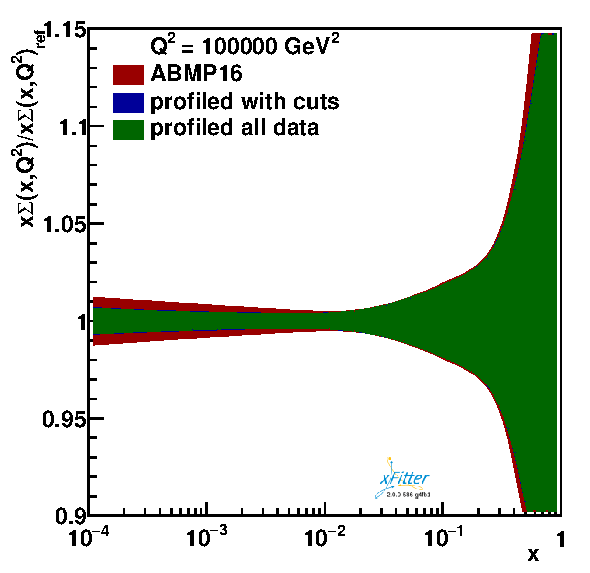
\includegraphics[width=0.235\textwidth]{pics/pdf-profile-ffabm/q2_100000_pdf_Sea_ratio.pdf}}}
    {{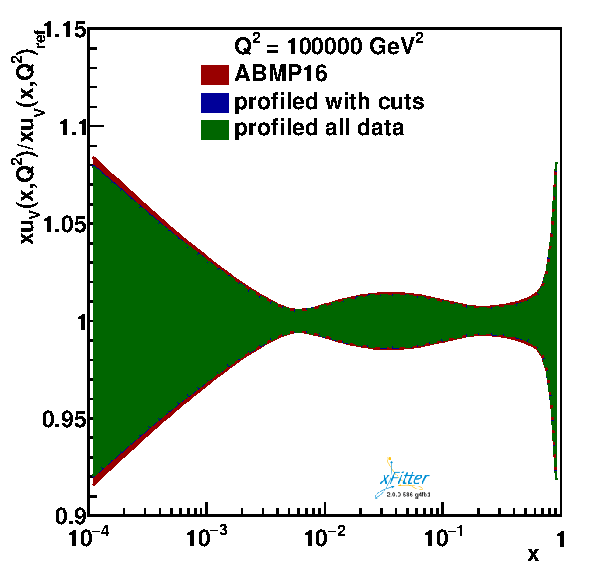
\includegraphics[width=0.235\textwidth]{pics/pdf-profile-ffabm/q2_100000_pdf_uv_ratio.pdf}}}
    {{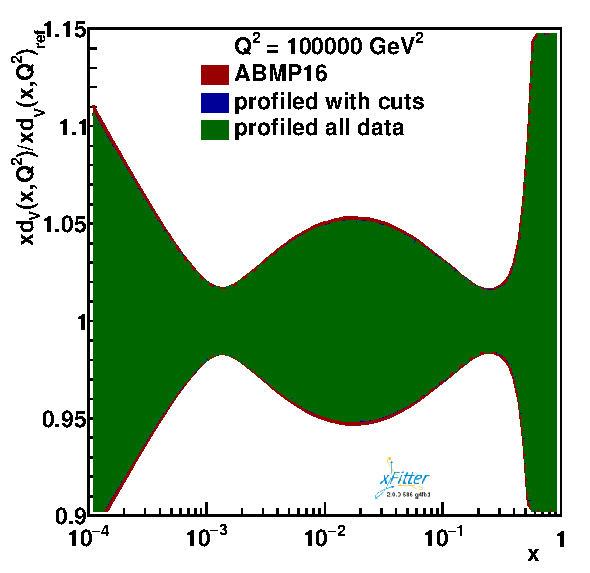
\includegraphics[width=0.235\textwidth]{pics/pdf-profile-ffabm/q2_100000_pdf_dv_ratio.pdf}}}
    \caption{The relative strange (top left), gluon (top right), sea quark (middle left), u valence quark (middle right) and d valence quark (bottom) PDF uncertainties at $\mu_\mathrm{f}^2=100000$ GeV$^2$ of the original and profiled \abmp PDF set.}
    \label{fig:pdf-abmp-100000}
\end{figure}

\begin{figure}
    \centering
    {{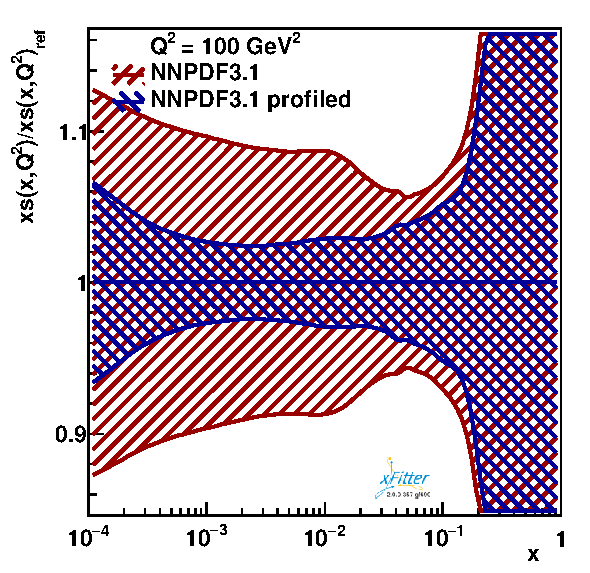
\includegraphics[width=0.235\textwidth]{pics/pdf-profile-fonll/q2_100_pdf_s_ratio.pdf}}}
    {{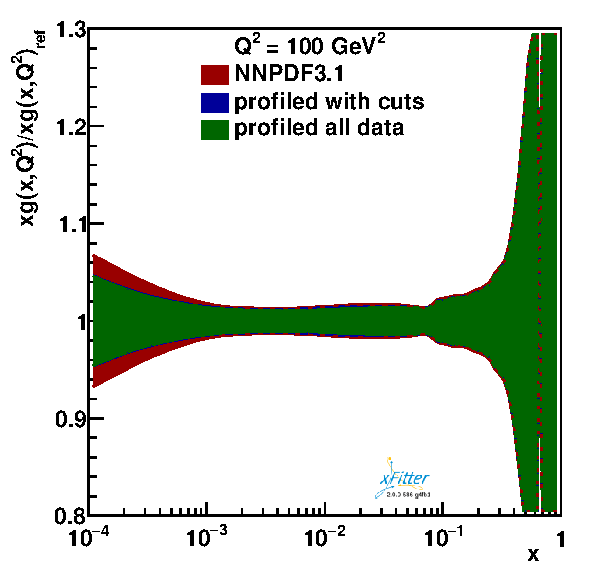
\includegraphics[width=0.235\textwidth]{pics/pdf-profile-fonll/q2_100_pdf_g_ratio.pdf}}}\\
    {{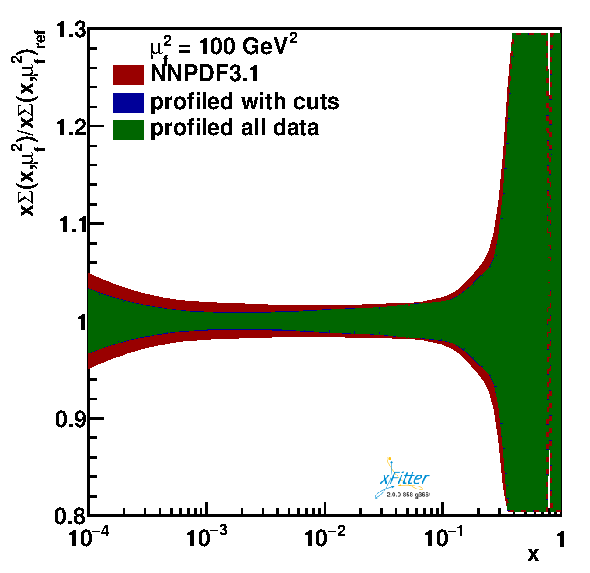
\includegraphics[width=0.235\textwidth]{pics/pdf-profile-fonll/q2_100_pdf_Sea_ratio.pdf}}}
    {{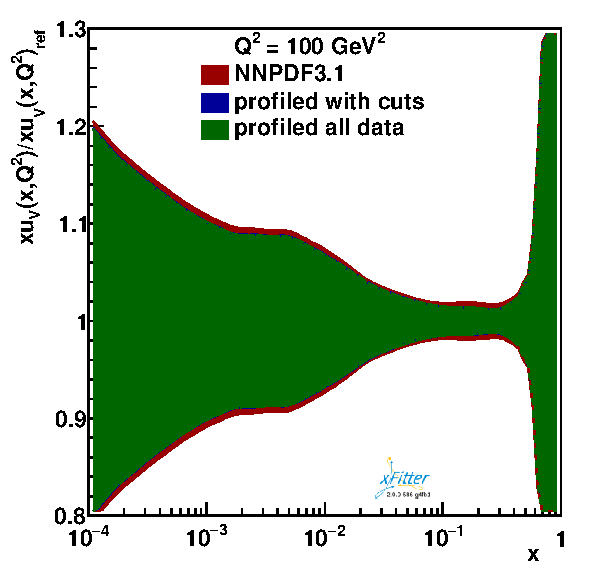
\includegraphics[width=0.235\textwidth]{pics/pdf-profile-fonll/q2_100_pdf_uv_ratio.pdf}}}
    {{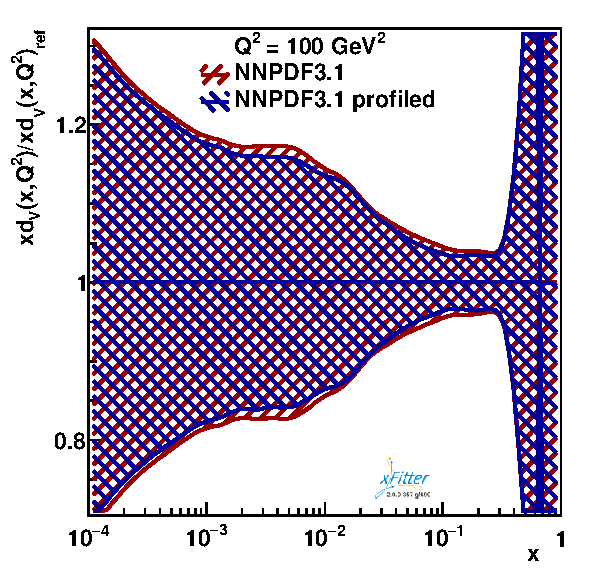
\includegraphics[width=0.235\textwidth]{pics/pdf-profile-fonll/q2_100_pdf_dv_ratio.pdf}}}
    {{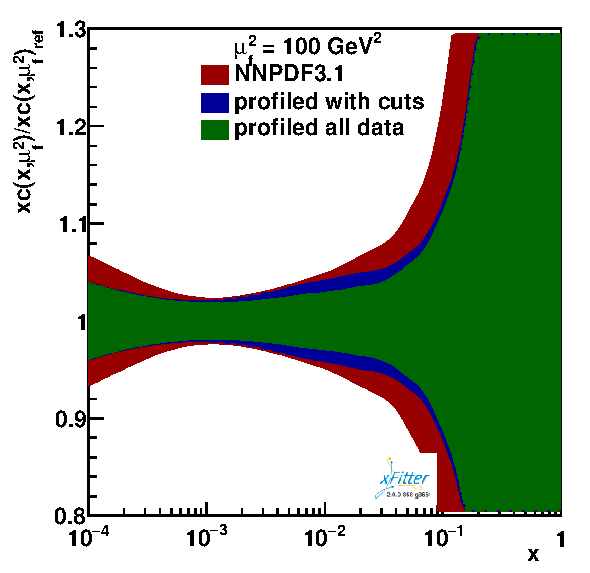
\includegraphics[width=0.235\textwidth]{pics/pdf-profile-fonll/q2_100_pdf_c_ratio.pdf}}}
    \caption{The relative strange (top left), gluon (top right), sea quark (middle left), u valence quark (middle right), d valence quark (bottom left) and charm quark (bottom right) PDF uncertainties at $\mu_\mathrm{f}^2=100$ GeV$^2$ of the original and profiled \nnpdf PDF set.}
    \label{fig:pdf-nnpdf}
\end{figure}

\begin{figure}
    \centering
    {{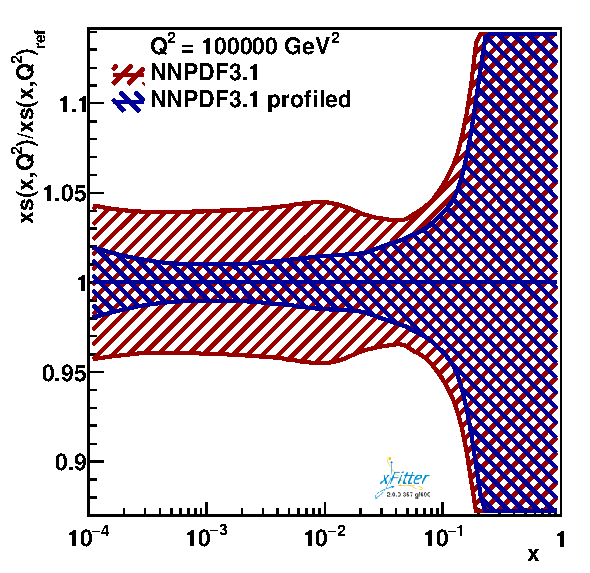
\includegraphics[width=0.235\textwidth]{pics/pdf-profile-fonll/q2_100000_pdf_s_ratio.pdf}}}
    {{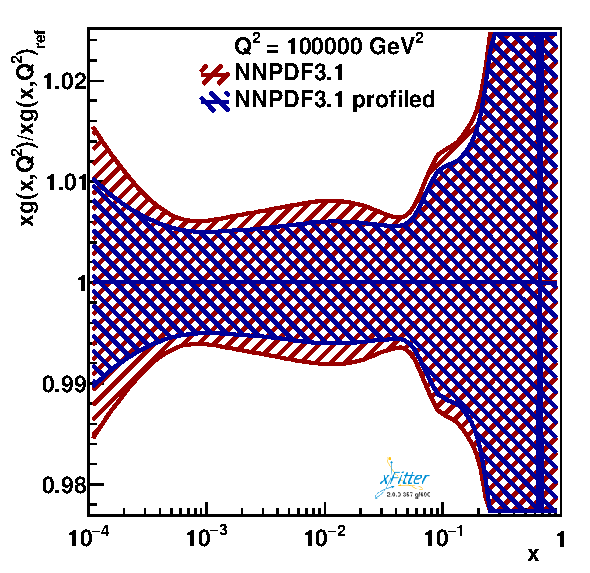
\includegraphics[width=0.235\textwidth]{pics/pdf-profile-fonll/q2_100000_pdf_g_ratio.pdf}}}\\
    {{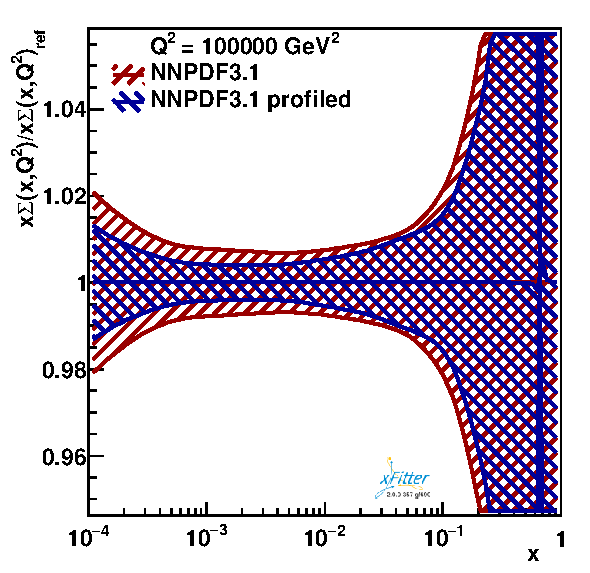
\includegraphics[width=0.235\textwidth]{pics/pdf-profile-fonll/q2_100000_pdf_Sea_ratio.pdf}}}
    {{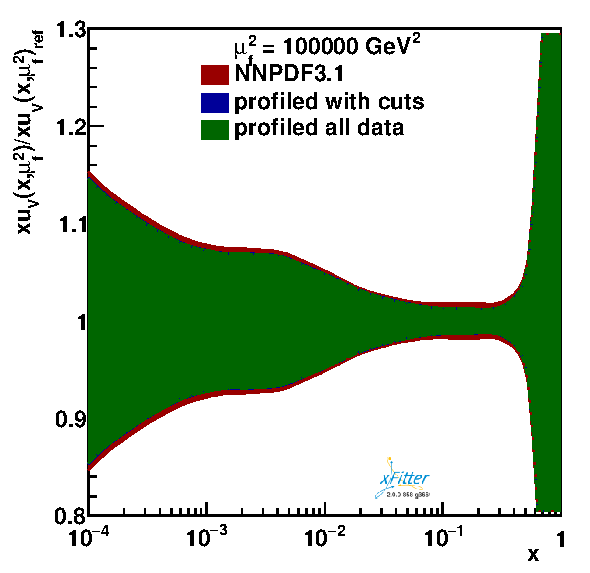
\includegraphics[width=0.235\textwidth]{pics/pdf-profile-fonll/q2_100000_pdf_uv_ratio.pdf}}}
    {{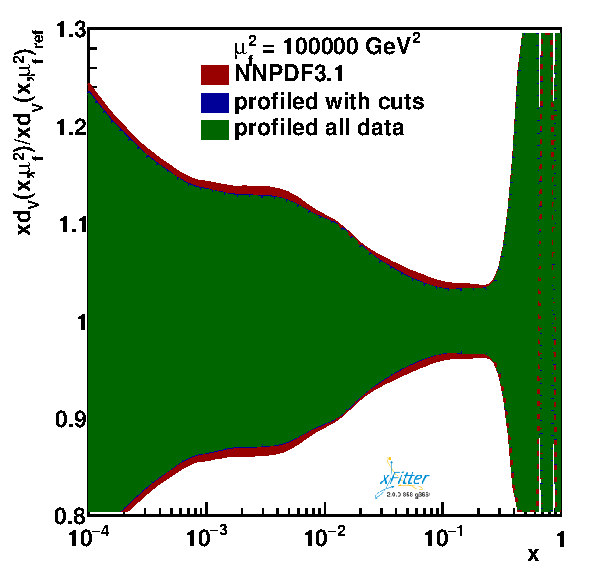
\includegraphics[width=0.235\textwidth]{pics/pdf-profile-fonll/q2_100000_pdf_dv_ratio.pdf}}}
    {{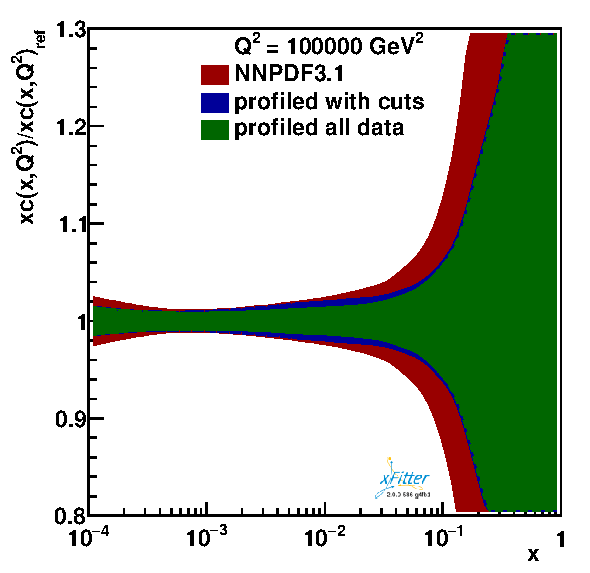
\includegraphics[width=0.235\textwidth]{pics/pdf-profile-fonll/q2_100000_pdf_c_ratio.pdf}}}
    \caption{The relative strange (top left), gluon (top right), sea quark (middle left), u valence quark (middle right), d valence quark (bottom left) and charm quark (bottom right) PDF uncertainties at $\mu_\mathrm{f}^2=100000$ GeV$^2$ of the original and profiled \nnpdf PDF set.}
    \label{fig:pdf-nnpdf-100000}
\end{figure}


\begin{acknowledgements}
%  We would like to thank Juan Rojo for a cri\-ti\-cal reading of this
%  paper, and Luca Rottoli for discussions on the description of charm
%  data.  V.~B.\ and F.~G.\ are supported by the European Research
%  Council Starting Grant ``PDF4BSM''.  Additional support was received
%  by A.~G., A.~S.\ and P.~S.\ from the BMBF-JINR cooperation program
%  and the Heisenberg-Landau program.  A.~L.\ is supported by the
%  Polish Ministry under program Mobility Plus, no 1320/MOB/IV/2015/0.
%  M.~B.\ is supported by the by the Marie Sk\l{}odowska Curie grant
%  HiPPiE@LHC.
\end{acknowledgements}

\section{Discussion and summary}

\bibliographystyle{spphys}
\bibliography{c_cpaper}

\end{document}
